\chapter{COMPARISON WITH POPULAR METHODS} \label{ch:comparison}% Must have a blank line after every section label

\epigraph{Comparison is the death of joy.}{Mark Twain}

\epigraph{Beware of bugs in the above code; I have only proved it correct, not tried it.}{Donald Knuth}



\noindent In this chapter, I apply the leximin algorithm to a set of common benchmark networks which vary in size and how well-defined their communities are. I evaluate the fitness of the leximin algorithm for community detection by ability to recover the ground-truth communities defined in the benchmark. I show that the leximin method is competitive with other methods on graphs with strong communities. In terms of the common accuracy measure, normalized mutual information (NMI), the leximin method achieves a higher community detection accuracy than all eight popular methods when communities are weak. This performance is an artifact of how NMI is computed, rather than an indication that the leximin method better recovers the true communities. I use this to argue that NMI should be replaced with adjusted mutual information (AMI). I show that large graphs with high connection between communities induce gridlock, and I show that the practical running time of the method is a hindrance from adoption.



\section{Introduction}

In real-world applications of community detection methods, the true clustering is unavailable. Instead, benchmarks have been proposed on which to evaluate these methods. These benchmark graphs have a known ground truth, so different measures of quality can be computed. When the method is applied to the benchmark graph, the identified clustering is compared against the ground truth. 



\subsection{LFR Benchmark Graphs}

Some real-world networks have been used to evaluate community detection~\cite{krebs2002mapping, padgett1993robust, zachary1977information, lusseau2003bottlenose}. The networks are few, which motivated creation of artificial networks with clear community structure. It is important that such artificial networks reflect properties of the networks they will be applied to. Four well-corroborated and agreed-upon properties of real networks are:
\begin{itemize}

\item sparsity: few connections between nodes,
\item power laws, 
\item small diameter (the \emph{small world effect}), and 
\item community effects~\cite{chakrabarti2006graph, barabasi2016network, chung2010graph, kolaczyk2014statistical}.
\end{itemize}

The $l$-planted partition model, and more specifically the Girvan--Newman (GN) benchmark, while commonplace, display only some of these characteristics. Many graphs for a given set of GN parameters can be created, and they generally display small diameter and community effects~\cite{condon2001algorithms, girvan2002community}. A GN benchmark is a graph on 128 nodes, divided into four equally-sized groups. Each of the four groups is a community to be identified. Every node has the same degree, and the \emph{mixing parameter}~$\mu$ controls the expected number of edges within the group, versus without. The mixing parameter is defined as
\begin{equation}  
\mu = \frac
{\sum_{v \in V}\deg^{inter}(v)}
{\sum_{v \in V}\deg(v)}
\end{equation}
and relates the inter-community degree~$\deg^{inter}(v)$ to the node's total degree~$\deg(v)$. Strong communities require that each node is more connected to its community than to others, so for $\mu > \frac{1}{2}$, strong communities cannot exist~\cite{yang2016comparative}.

As long as $\mu$ is less than 0.5, most edges are between members of the same community, so communities should be identifiable. The GN benchmark does not represent real-world graphs, though. There is no variation in node degree or community size, and the network size is small.

The LFR benchmark graphs (named for the designers) better reflect real-world graphs, and they are a harder test. They have power-law (or \emph{scale-free}) distributions of node degree and community size. Like the GN test, their connectivity structures are not entirely prescribed by their parameters. Instead, a configuration model is used to create graphs satisfying the given constraints. Also like the GN test, the strength of communities is controlled by a global mixing parameter~$\mu$, and above $\mu = \frac{1}{2}$, strong communities cannot exist. Yang et al.\ showed the importance of the mixing parameter~$\mu$ as a determiner of the accuracy of community detection; we use their framework to assess the quality of community detection.



\section{Experimental Setup}

\begin{table}
	\centering
	\caption{Parameter grid for LFR benchmark graphs}
		\begin{tabular}{l r}
		\toprule
		Parameter & Value \\
		\midrule
		Number of nodes $N$ & $\numrange{80}{240}$ \\
		Maximum degree & $0.2N$ \\
		Maximum community size & $0.2N$ \\
		Average degree & $10$ \\
		Degree distribution exponent & $-2$ \\
		Community size distribution exponent & $-1$ \\
		Mixing coefficient $\mu$ & $\numrange{0.03}{0.75}$ \\
		\bottomrule
		\end{tabular}
	\label{tab:Parameter grid}
\end{table}

\begin{table}
	\centering
	\caption{Properties of community detection methods under consideration. The speed classifications of the first eight methods are those presented by Yang et al.~\cite{yang2016comparative}.}
	\begin{tabular}{l l l l}
	\toprule
	Method & Speed & Hierarchical? & Style \\
	\midrule
	Edge betweenness (GN) & Slow & Y & Divisive \\
	Fastgreedy & Fast & Y & Agglomerative \\
	Infomap & Fast & N \\
	Label propagation (LPA) & Fast & N \\
	Leading eigenvector & Fast & Y & Divisive\\
	Multilevel & Fast & N \\
	Spinglass & Slow & N \\
	Walktrap & Fast & Y & Agglomerative \\
	\textbf{Leximin} & \textbf{Slow} & \textbf{Y} & \textbf{Divisive} \\
	\bottomrule
	\end{tabular}
	
	\label{tab:methods}
\end{table}

We follow the methodology of Yang et al.~\cite{yang2016comparative} to compare the leximin method's accuracy to other methods. This model has been adopted by other researchers to contextualize new community detection algorithms~\cite{pares2017fluid}. Holding all other parameters fixed, we create 25 LFR benchmark graphs each for a spread of network sizes and $\mu$~values. We evaluate each algorithm's ability to recover the communities produced by the LFR benchmark.

The parameters we used are given in \autoref{tab:Parameter grid}.
This parameterization of the model largely aligns with the work of Yang et al.~\cite{yang2016comparative}. Due to the temporal constraints of the maximin algorithm, the average degree and network size parameters needed to be reduced. The community size and degree distribution exponents are preserved at~$-1$ and~$-2$ respectively, in line with Lancichinetti et al.~\cite{lancichinetti2008benchmark}.

Yang et al.~\cite{yang2016comparative} compare the following methods' performance across various facets: Fastgreedy~\cite{clauset2004finding}, Infomap~\cite{rosvall2007information, rosvall2009map}, label propagation~\cite{raghavan2007near}, leading eigenvector~\cite{newman2006finding}, multilevel~\cite{blondel2008fast}, spinglass~\cite{reichardt2006statistical}, and walktrap~\cite{pons2005computing}. The key properties of each algorithm, along with the maximin algorithm, are given in \autoref{tab:methods}. For a concise description of each method, the reader is directed to Yang et al.~\cite{yang2016comparative}.

The leximin method is implemented in AMPL~\cite{fourer1989mathematical}. Using AMPL's CPLEX backend~\cite{cplex2009v12}, the method solves the LP of Dong et al.'s \emph{triples} formulation of the MCFP~\cite{dong2015compact}. The eight other algorithms are implemented in the \say{igraph} package, accessed through \say{igraph}'s R interface. Determining optimal modularity is built-in for the \say{igraph} algorithms; it is done using the \say{networkx} Python library~\cite{hagberg2008exploring} for leximin. Cluster evaluation is done for all using the NMI and AMI functions of the \say{scikit-learn} Python package~\cite{pedregosa2011scikit}.



\section{Results}

To compare the communities identified by the various algorithms to the true communities, Yang et al.\ used two measures:  the \emph{normalized mutual information} (NMI) and the ratio of the number of identified communities to the number of communities given by the LFR model. We use the results of our analysis to argue that NMI should be supplanted by a newer metric, \emph{adjusted mutual information} (AMI). We compare the performance of each method, using these three measures, for varying network size and $\mu$.



\subsection{Effect of Network Mixing Parameter on Accuracy}

\begin{figure}
  \centering

    \begin{subfigure}[b]{0.32\textwidth}
        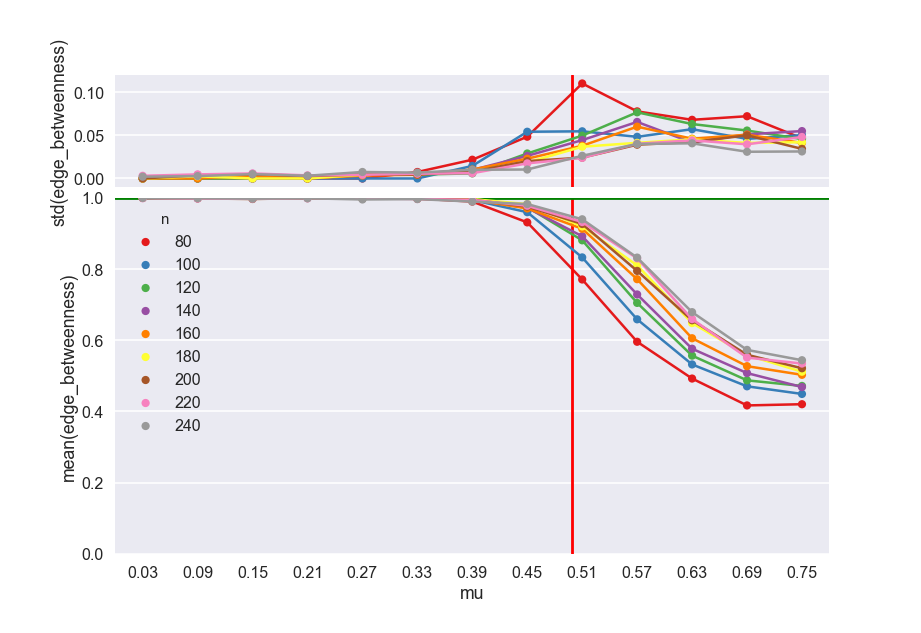
\includegraphics[width=\textwidth]{fig/nmi_vs_mu_edge_betweenness}
        \caption{Edge betweenness (GN)}
        \label{fig:gull}
    \end{subfigure}
    \qquad%add desired spacing between images, e. g. ~, \quad, \qquad, \hfill etc. 
      %(or a blank line to force the subfigure onto a new line)
    \begin{subfigure}[b]{0.32\textwidth}
        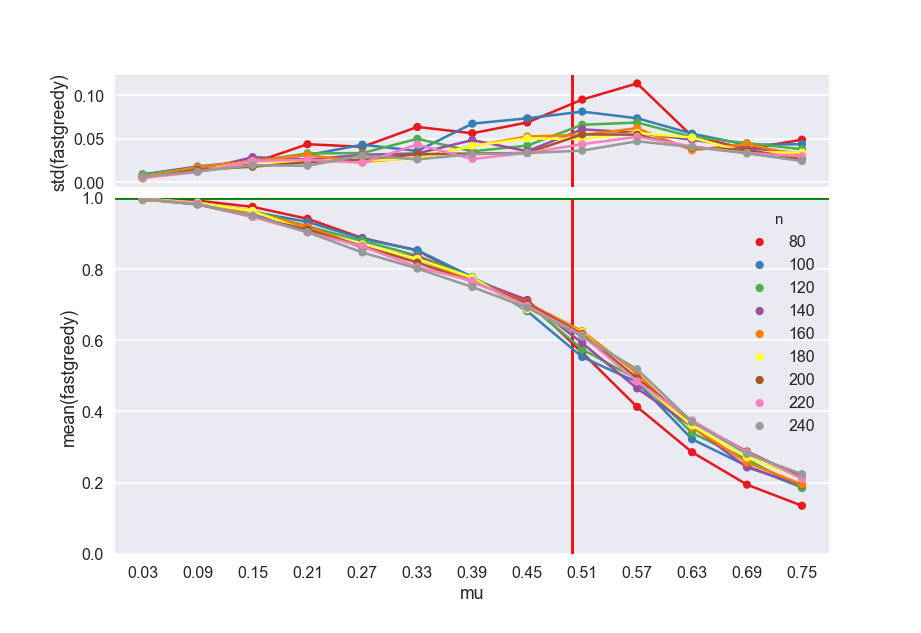
\includegraphics[width=\textwidth]{fig/nmi_vs_mu_fastgreedy}
        \caption{Fastgreedy}
        \label{fig:tiger}
    \end{subfigure}
    %add desired spacing between images, e. g. ~, \quad, \qquad, \hfill etc. 
    %(or a blank line to force the subfigure onto a new line)
    
    \begin{subfigure}[b]{0.32\textwidth}
        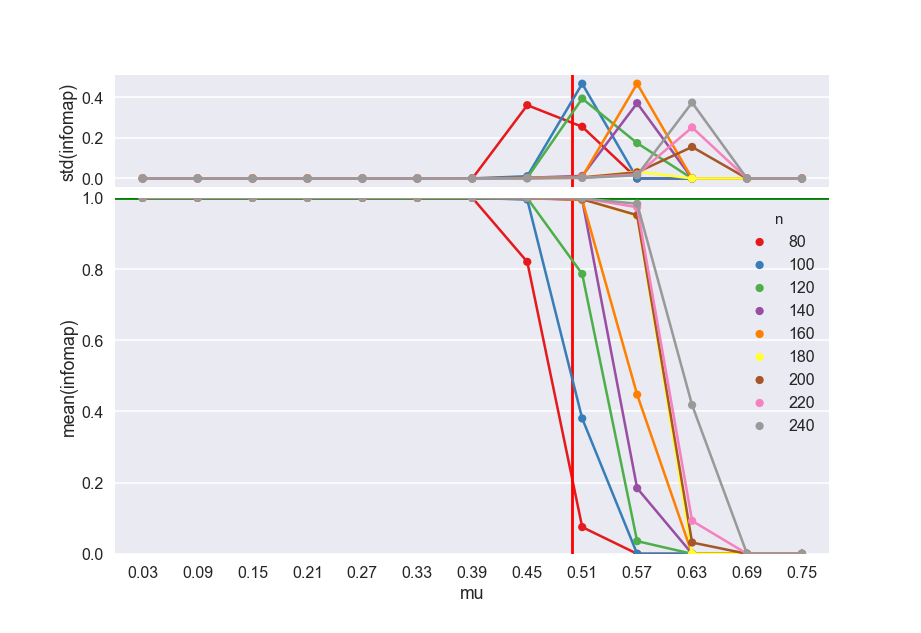
\includegraphics[width=\textwidth]{fig/nmi_vs_mu_infomap}
        \caption{Infomap}
        \label{fig:mouse}
    \end{subfigure}
    \qquad
    \begin{subfigure}[b]{0.32\textwidth}
        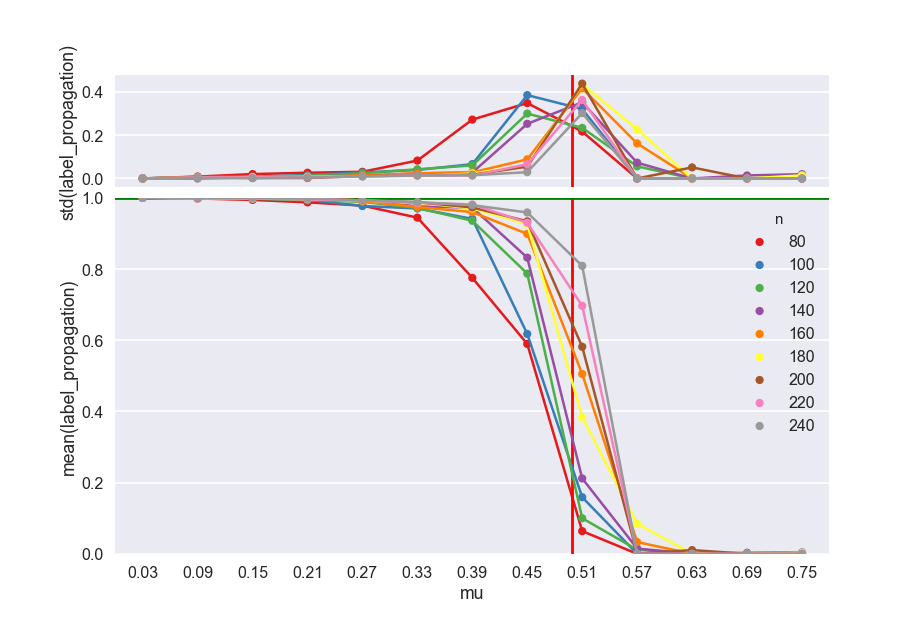
\includegraphics[width=\textwidth]{fig/nmi_vs_mu_label_propagation}
        \caption{Label propagation (LPA)}
        \label{fig:gull}
    \end{subfigure}
    %add desired spacing between images, e. g. ~, \quad, \qquad, \hfill etc. 
      %(or a blank line to force the subfigure onto a new line)
      
    \begin{subfigure}[b]{0.32\textwidth}
        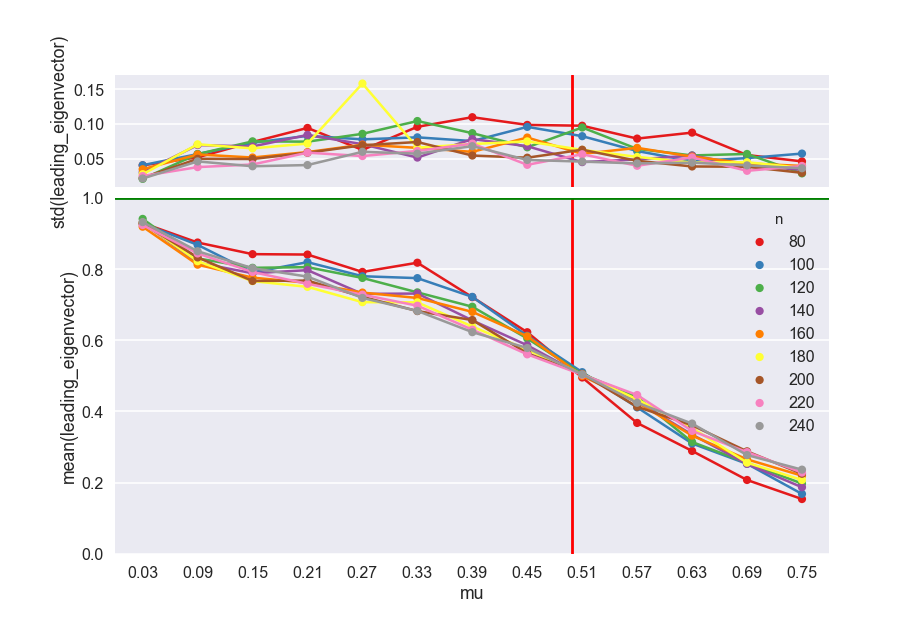
\includegraphics[width=\textwidth]{fig/nmi_vs_mu_leading_eigenvector}
        \caption{Leading eigenvector}
        \label{fig:tiger}
    \end{subfigure}
    \qquad
    %add desired spacing between images, e. g. ~, \quad, \qquad, \hfill etc. 
    %(or a blank line to force the subfigure onto a new line)
    \begin{subfigure}[b]{0.32\textwidth}
        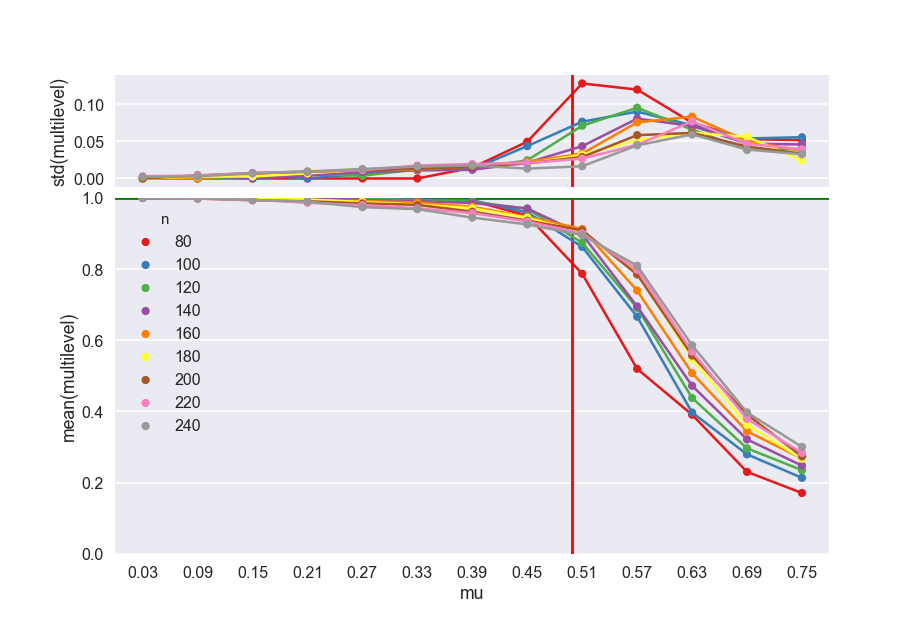
\includegraphics[width=\textwidth]{fig/nmi_vs_mu_multilevel}
        \caption{Multilevel}
        \label{fig:mouse}
    \end{subfigure}

    \begin{subfigure}[b]{0.32\textwidth}
        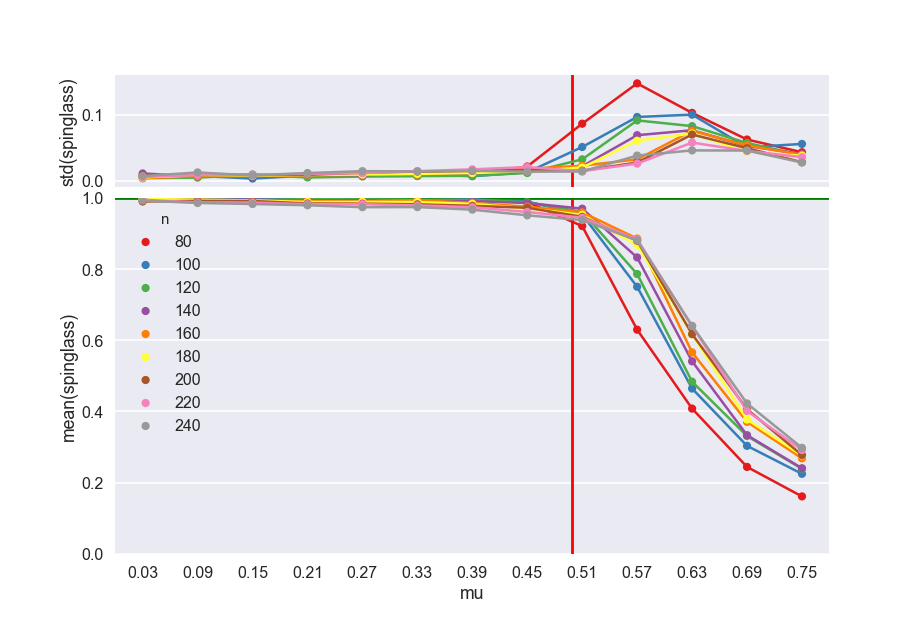
\includegraphics[width=\textwidth]{fig/nmi_vs_mu_spinglass}
        \caption{Spinglass}
        \label{fig:gull}
    \end{subfigure}
    \qquad
    %add desired spacing between images, e. g. ~, \quad, \qquad, \hfill etc. 
      %(or a blank line to force the subfigure onto a new line)
    \begin{subfigure}[b]{0.32\textwidth}
        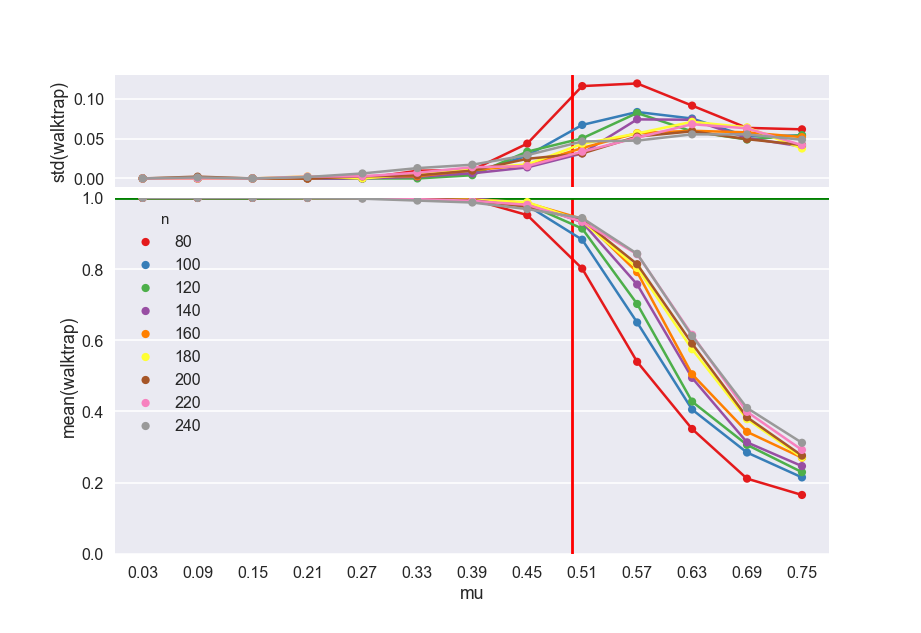
\includegraphics[width=\textwidth]{fig/nmi_vs_mu_walktrap}
        \caption{Walktrap}
        \label{fig:tiger}
    \end{subfigure}
    
    %add desired spacing between images, e. g. ~, \quad, \qquad, \hfill etc. 
    %(or a blank line to force the subfigure onto a new line)
    \begin{subfigure}[b]{0.32\textwidth}
        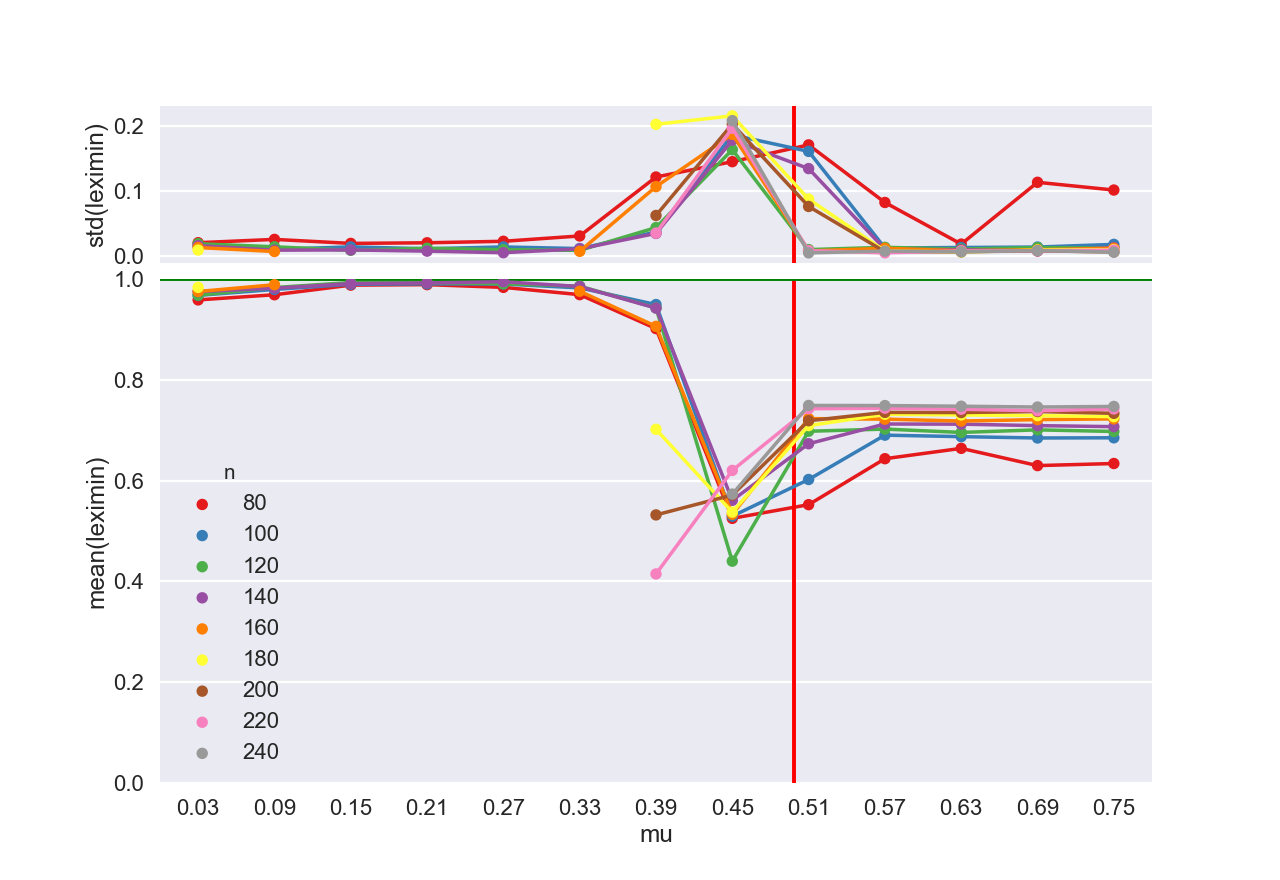
\includegraphics[width=\textwidth]{fig/nmi_vs_mu_leximin}
        \caption{Leximin}
        \label{fig:mouse}
    \end{subfigure}

  \caption{The mean (top) and standard deviation (bottom) of normalized mutual information~(NMI) as a function of the mixing parameter,~$\mu$. Please note that the vertical axis range may differ across plots. The different colors represent different network sizes. The vertical line indicates the boundary between strong and weak communities, $\mu = 0.5$.}
  \label{fig:mu_nmi}
\end{figure}

First, we examine how the strength of community ties affects the accuracy of the leximin method. The first measure we use is normalized mutual information (NMI). NMI is a concept from information theory that has been commonly used to appraise agreement between communities~\cite{danon2005comparing}. This metric is independent of the values of the labels: a permutation of the community labels won't change the score in any way.

\begin{table}
  \centering
  \caption{A contingency table for the leximin method on an LFR graph with 80 nodes. Six communities are defined according to the benchmark generator. The leximin method identifies nine, though three of these only contain a single node (communities A, F, and H). The true communities 1, 3, 4, and 6 are perfectly recovered as communities E, C, D, and B, respectively.}
  \begin{tabular}{l|rrrrrrrrr}
  \toprule
  predicted &  A &   B &  C &   D &   E &  F &   G &  H &   I \\
  true &    &     &    &     &     &    &     &    &     \\
  \midrule
  1    &  0 &   0 &  0 &   0 &  \textbf{12} &  0 &   0 &  0 &   0 \\
  2    &  \textbf{1} &   0 &  0 &   0 &   0 &  0 &   0 &  0 &  \textbf{15} \\
  3    &  0 &   0 &  \textbf{8} &   0 &   0 &  0 &   0 &  0 &   0 \\
  4    &  0 &   0 &  0 &  \textbf{15} &   0 &  0 &   0 &  0 &   0 \\
  5    &  0 &   0 &  0 &   0 &   0 &  \textbf{1} &  \textbf{15} &  \textbf{1} &   0 \\
  6    &  0 &  \textbf{12} &  0 &   0 &   0 &  0 &   0 &  0 &   0 \\
  \bottomrule
  \end{tabular}
  \label{tab:crosstab}
\end{table}

NMI is calculated from the contingency table (or \say{cross tabulation})~$T$, a tool to assess misclassifications. An example is provided in \autoref{tab:crosstab}. It has one row for each true community and one column for each detected community, and the $\{i,j\}$th entry is the number of nodes in community $i$ that were marked as members of community $j$. NMI is computed as
\begin{equation}
\mathrm{NMI} = \frac
{-2\sum_{i=1}^{C} \sum_{j=1}^{\overline{C}} T_{ij} \log(T_{ij} T/T_{io}T_{oj})}
{\sum_{i=1}^C T_{io} \log(T_{io}/T) + \sum_{j=1}^{\overline{C}} T_{oj} \log(T_{oj}/T)}
\end{equation}
where the number of true communities is $C$, the number of detected communities is $\overline{C}$, and $o$ represents a sum over a column or row. The values range from 1 for a perfect matching to 0 for a totally independent identified partition. 

The performance is shown in \autoref{fig:mu_nmi}. Each plot shows the performance of one algorithm. The lower subplot shows the mean NMI over 25 trials, and the upper plot shows the standard deviation. The performance of the leximin method is competitive for low $\mu$, but drops rapidly as communities become weaker. This behavior is exhibited by other methods, but other algorithms' sharp drops in accuracy occur at higher values of $\mu$. Unusually, the leximin method's performance ticks back upward for strong communities. The method achieves higher NMI than any other method for all high values of $\mu$. 

\begin{figure}
  \centering

    \begin{subfigure}[b]{0.32\textwidth}
        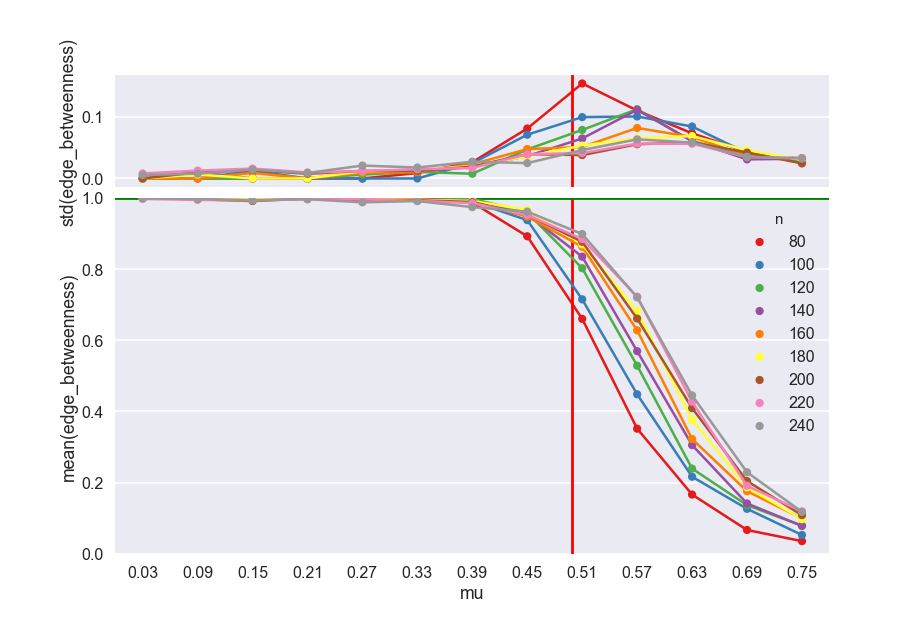
\includegraphics[width=\textwidth]{fig/ami_vs_mu_edge_betweenness}
        \caption{Edge betweenness (GN)}
        \label{fig:gull}
    \end{subfigure}
    \qquad
    %add desired spacing between images, e. g. ~, \quad, \qquad, \hfill etc. 
      %(or a blank line to force the subfigure onto a new line)
    \begin{subfigure}[b]{0.32\textwidth}
        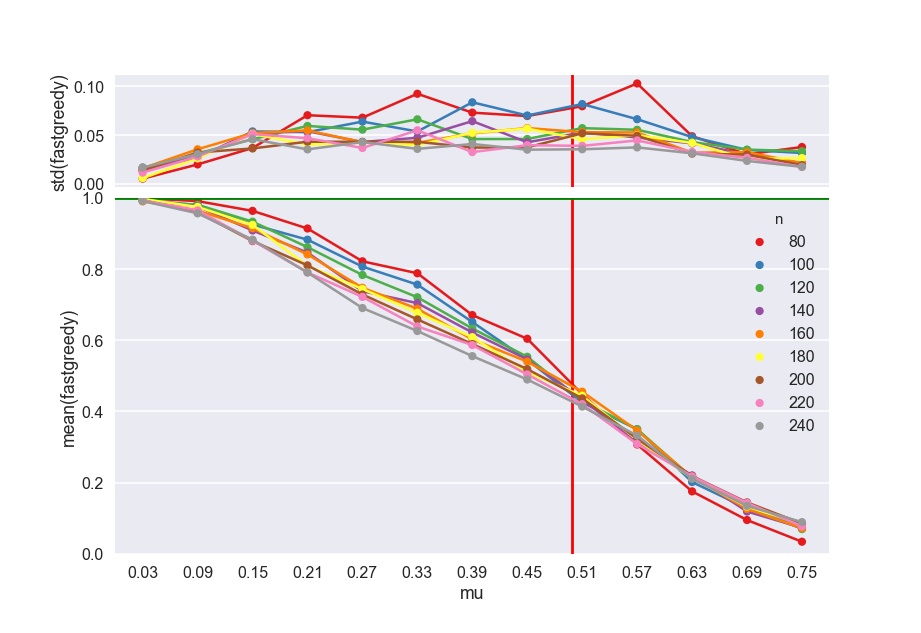
\includegraphics[width=\textwidth]{fig/ami_vs_mu_fastgreedy}
        \caption{Fastgreedy}
        \label{fig:tiger}
    \end{subfigure}
    
    %add desired spacing between images, e. g. ~, \quad, \qquad, \hfill etc. 
    %(or a blank line to force the subfigure onto a new line)
    \begin{subfigure}[b]{0.32\textwidth}
        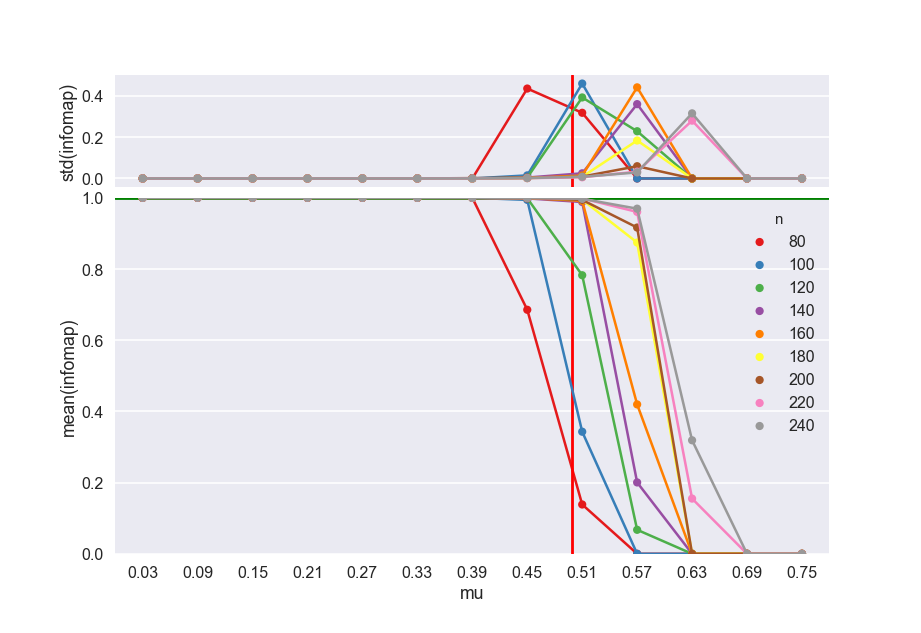
\includegraphics[width=\textwidth]{fig/ami_vs_mu_infomap}
        \caption{Infomap}
        \label{fig:mouse}
    \end{subfigure}
	\qquad
    \begin{subfigure}[b]{0.32\textwidth}
        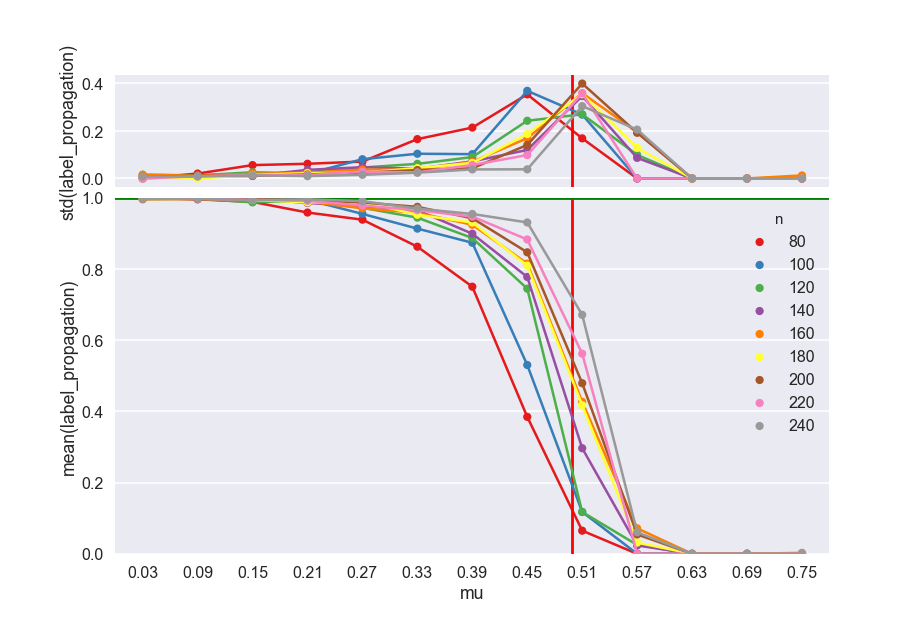
\includegraphics[width=\textwidth]{fig/ami_vs_mu_label_propagation}
        \caption{Label propagation (LPA)}
        \label{fig:gull}
    \end{subfigure}
    %add desired spacing between images, e. g. ~, \quad, \qquad, \hfill etc. 
      %(or a blank line to force the subfigure onto a new line)
      
    \begin{subfigure}[b]{0.32\textwidth}
        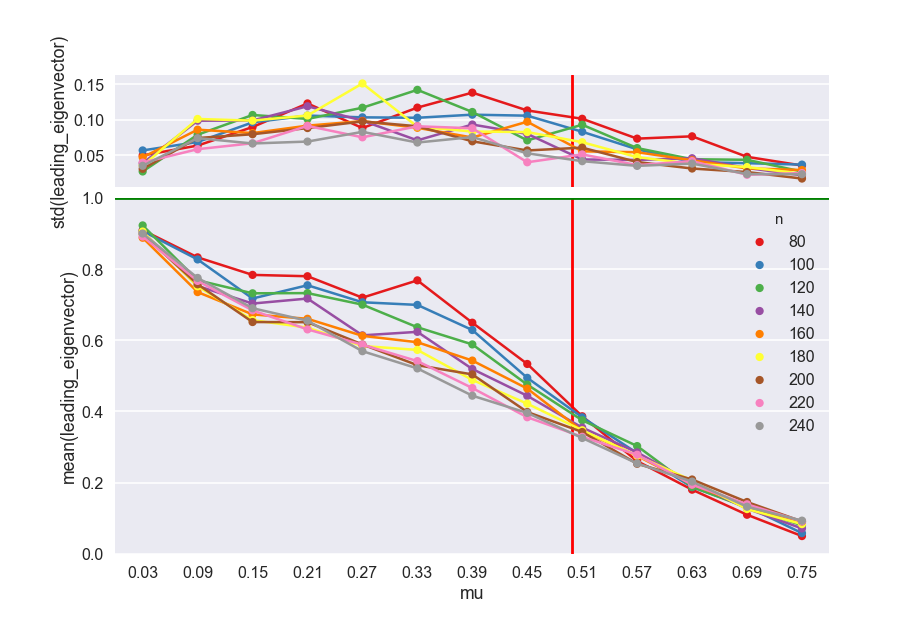
\includegraphics[width=\textwidth]{fig/ami_vs_mu_leading_eigenvector}
        \caption{Leading eigenvector}
        \label{fig:tiger}
    \end{subfigure}
    \qquad
    %add desired spacing between images, e. g. ~, \quad, \qquad, \hfill etc. 
    %(or a blank line to force the subfigure onto a new line)
    \begin{subfigure}[b]{0.32\textwidth}
        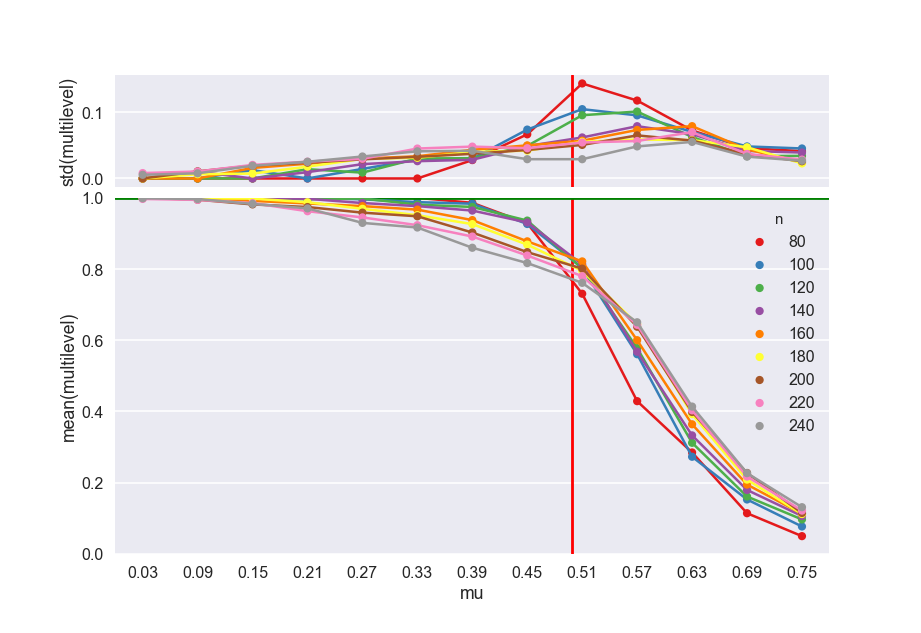
\includegraphics[width=\textwidth]{fig/ami_vs_mu_multilevel}
        \caption{Multilevel}
        \label{fig:mouse}
    \end{subfigure}
    
    \begin{subfigure}[b]{0.32\textwidth}
        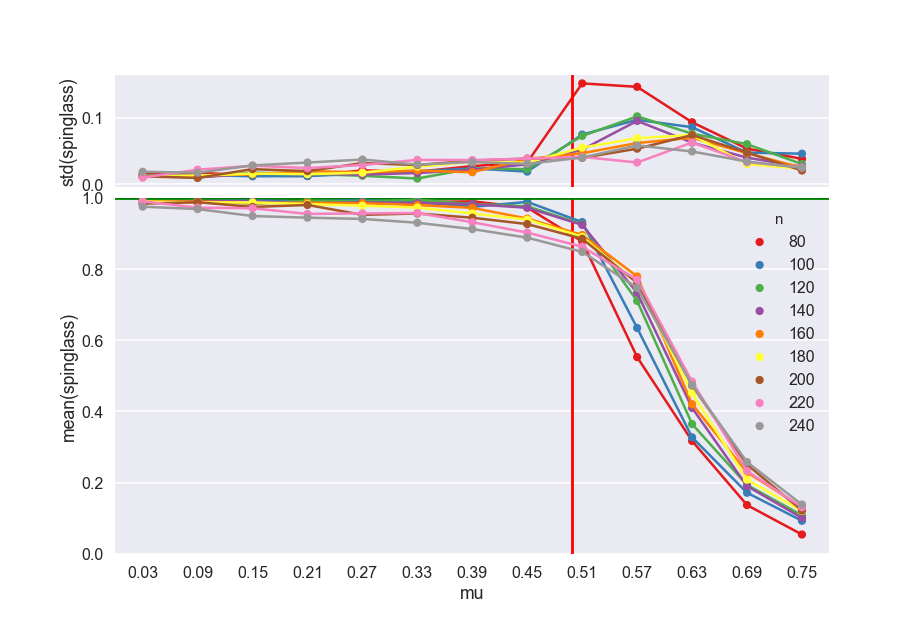
\includegraphics[width=\textwidth]{fig/ami_vs_mu_spinglass}
        \caption{Spinglass}
        \label{fig:gull}
    \end{subfigure}
    \qquad
    %add desired spacing between images, e. g. ~, \quad, \qquad, \hfill etc. 
      %(or a blank line to force the subfigure onto a new line)
    \begin{subfigure}[b]{0.32\textwidth}
        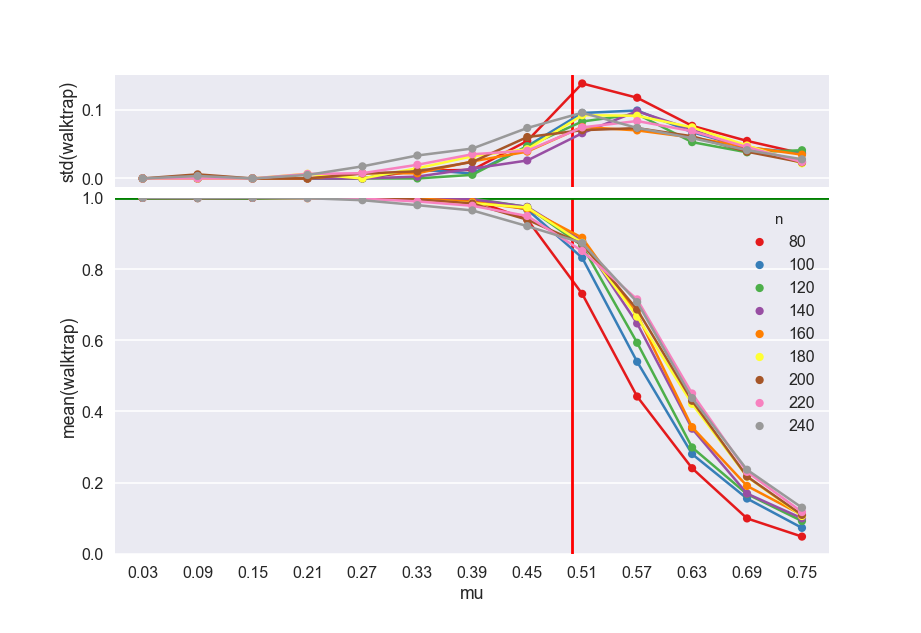
\includegraphics[width=\textwidth]{fig/ami_vs_mu_walktrap}
        \caption{Walktrap}
        \label{fig:tiger}
    \end{subfigure}
    
    %add desired spacing between images, e. g. ~, \quad, \qquad, \hfill etc. 
    %(or a blank line to force the subfigure onto a new line)
    \begin{subfigure}[b]{0.32\textwidth}
        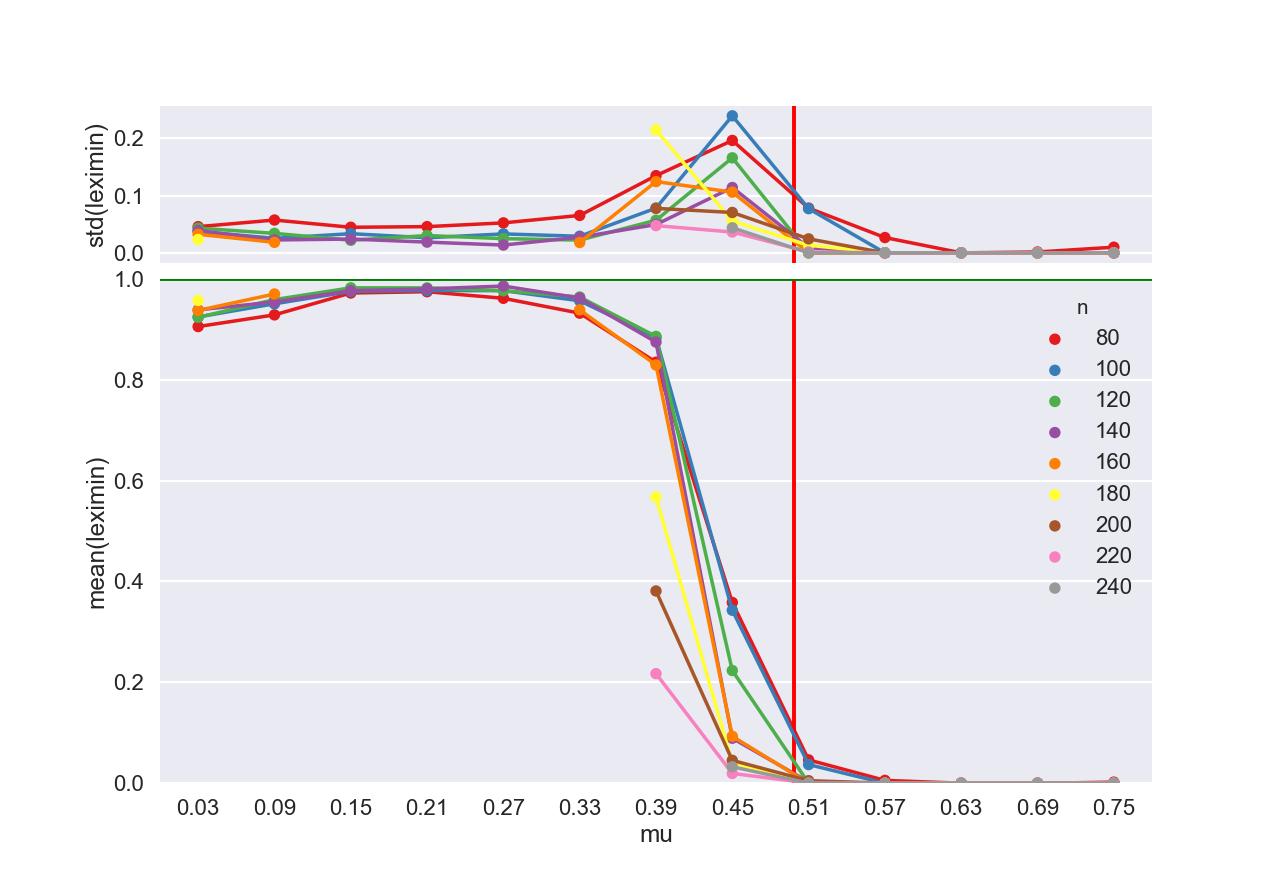
\includegraphics[width=\textwidth]{fig/ami_vs_mu_leximin}
        \caption{Leximin}
        \label{fig:mouse}
    \end{subfigure}

  \caption{The mean (top) and standard deviation (bottom) of adjusted mutual information~(AMI) as a function of the mixing parameter,~$\mu$. Please note that the vertical axis range may differ across plots. The different colors represent different network sizes. The vertical line indicates the boundary between strong and weak communities, $\mu = 0.5$.}
  \label{fig:mu_ami}
\end{figure}

This unusual behavior raises questions. These questions can be partially addressed by using adjusted mutual information (AMI) as the accuracy score. AMI is a recently proposed adjustment to NMI which discounts chance agreements of clusterings~\cite{vinh2009information}. The upper value is still 1, for a perfect agreement between true and computed clusterings. An AMI of~0 means performance equal to a chance assignment, which is achieved when each node is assigned to a unique cluster. Negative values indicate a computed clustering that is worse than chance.

The performance of all nine algorithms measured by AMI is shown in~\autoref{fig:mu_ami}. While most algorithms' accuracy is not notably different from the NMI measure, the leximin method's AMI drops to zero for large values of~$\mu$. This suggests that the strong NMI scores in this range are attributable to chance.

\begin{figure}
\centering
    \begin{subfigure}[b]{0.32\textwidth}
        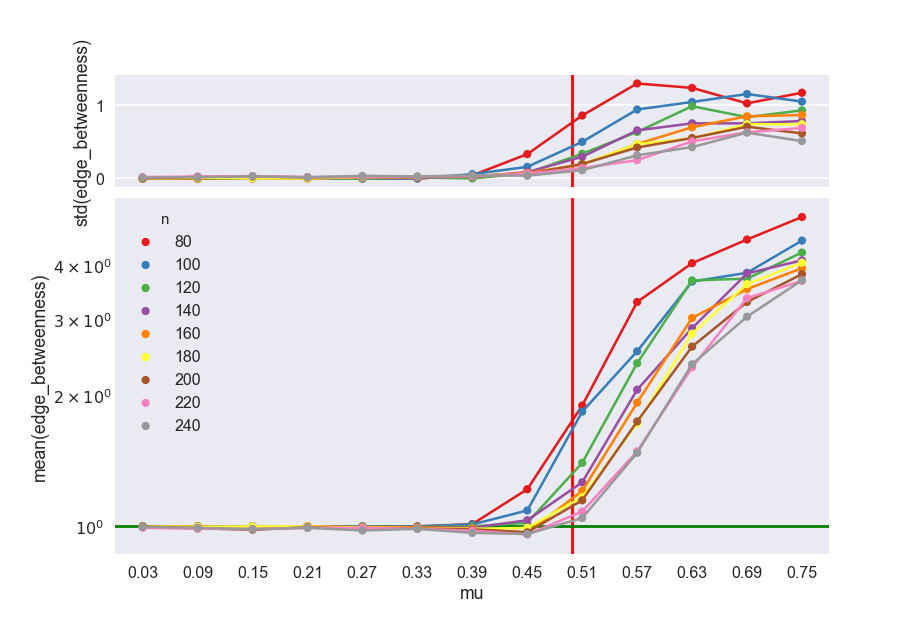
\includegraphics[width=\textwidth]{fig/ratio_vs_mu_edge_betweenness}
        \caption{Edge betweenness (GN)}
        \label{fig:gull}
    \end{subfigure}
    %add desired spacing between images, e. g. ~, \quad, \qquad, \hfill etc. 
      %(or a blank line to force the subfigure onto a new line)
    \qquad
    \begin{subfigure}[b]{0.32\textwidth}
        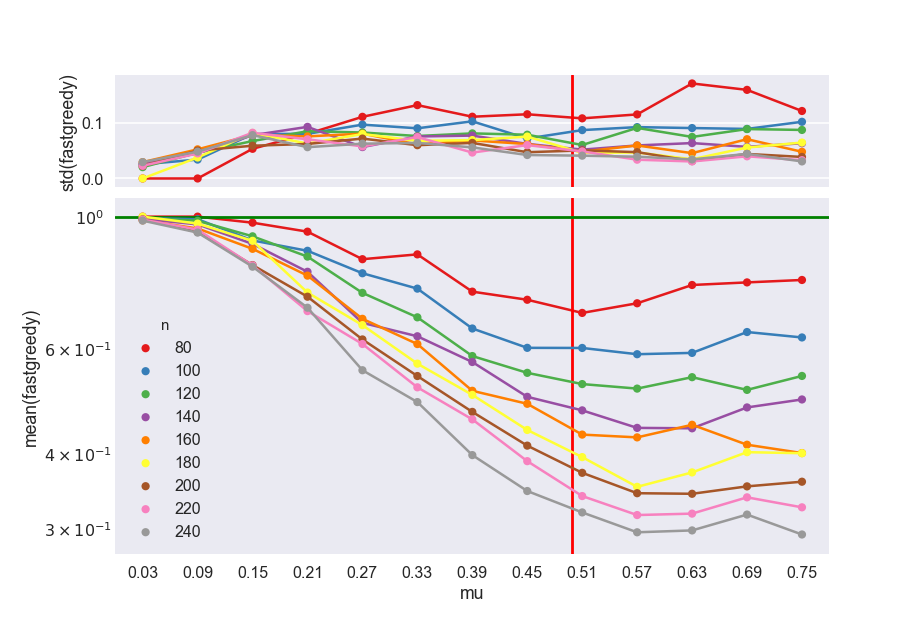
\includegraphics[width=\textwidth]{fig/ratio_vs_mu_fastgreedy}
        \caption{Fastgreedy}
        \label{fig:tiger}
    \end{subfigure}
    
    %add desired spacing between images, e. g. ~, \quad, \qquad, \hfill etc. 
    %(or a blank line to force the subfigure onto a new line)
    \begin{subfigure}[b]{0.32\textwidth}
        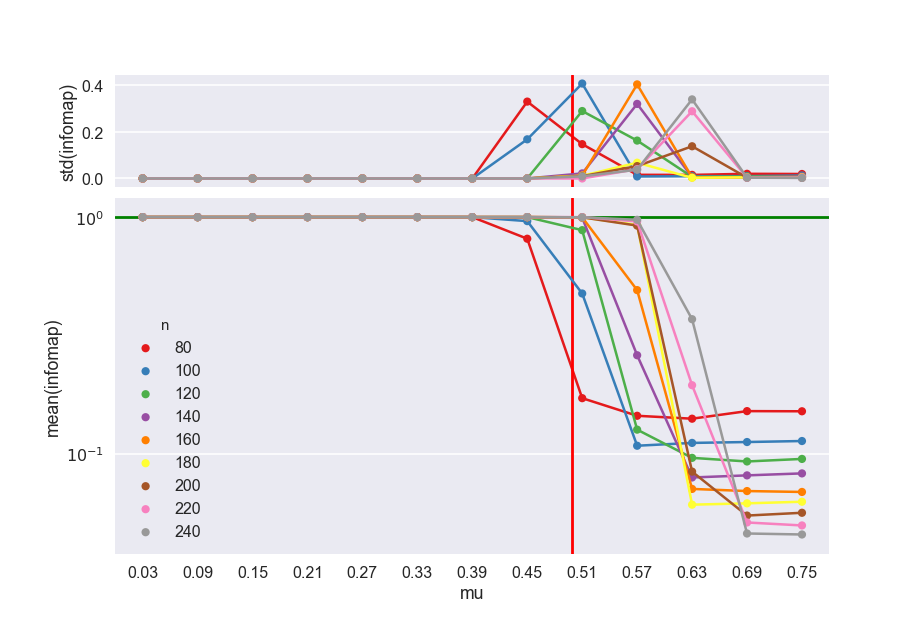
\includegraphics[width=\textwidth]{fig/ratio_vs_mu_infomap}
        \caption{Infomap}
        \label{fig:mouse}
    \end{subfigure}
    \qquad
    \begin{subfigure}[b]{0.32\textwidth}
        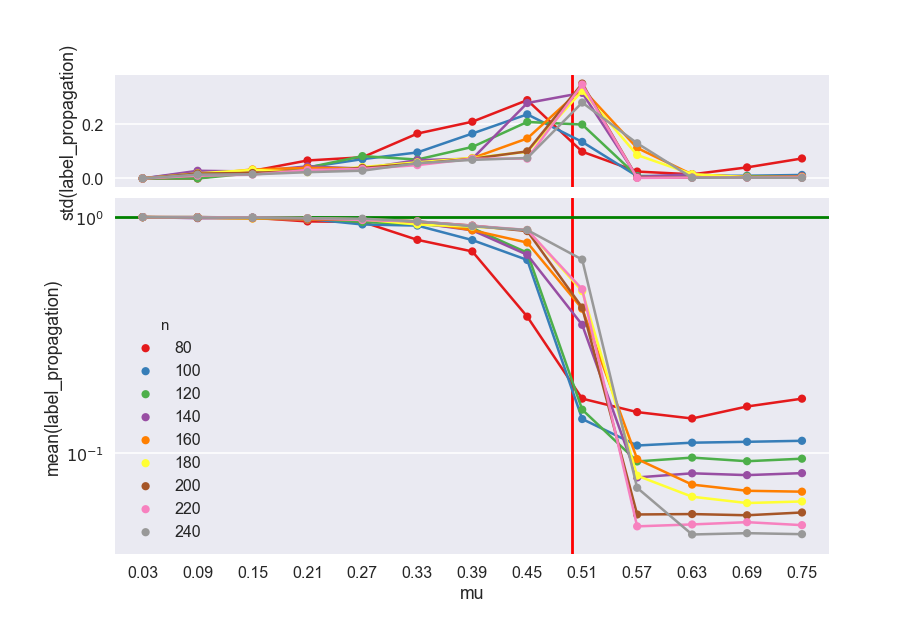
\includegraphics[width=\textwidth]{fig/ratio_vs_mu_label_propagation}
        \caption{Label propagation (LPA)}
        \label{fig:gull}
    \end{subfigure}
    %add desired spacing between images, e. g. ~, \quad, \qquad, \hfill etc. 
      %(or a blank line to force the subfigure onto a new line)
      
    \begin{subfigure}[b]{0.32\textwidth}
        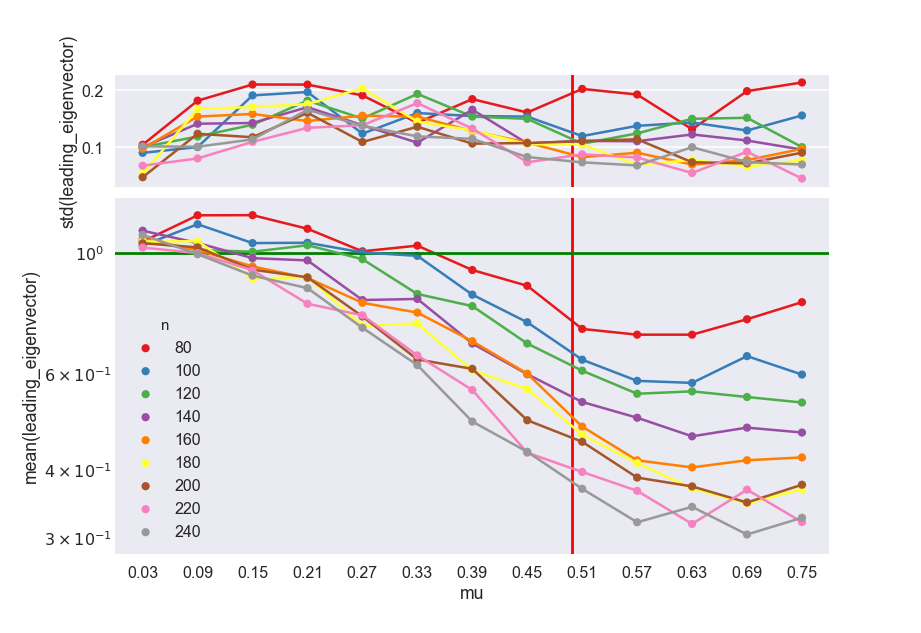
\includegraphics[width=\textwidth]{fig/ratio_vs_mu_leading_eigenvector}
        \caption{Leading eigenvector}
        \label{fig:tiger}
    \end{subfigure}
    \qquad
    %add desired spacing between images, e. g. ~, \quad, \qquad, \hfill etc. 
    %(or a blank line to force the subfigure onto a new line)
    \begin{subfigure}[b]{0.32\textwidth}
        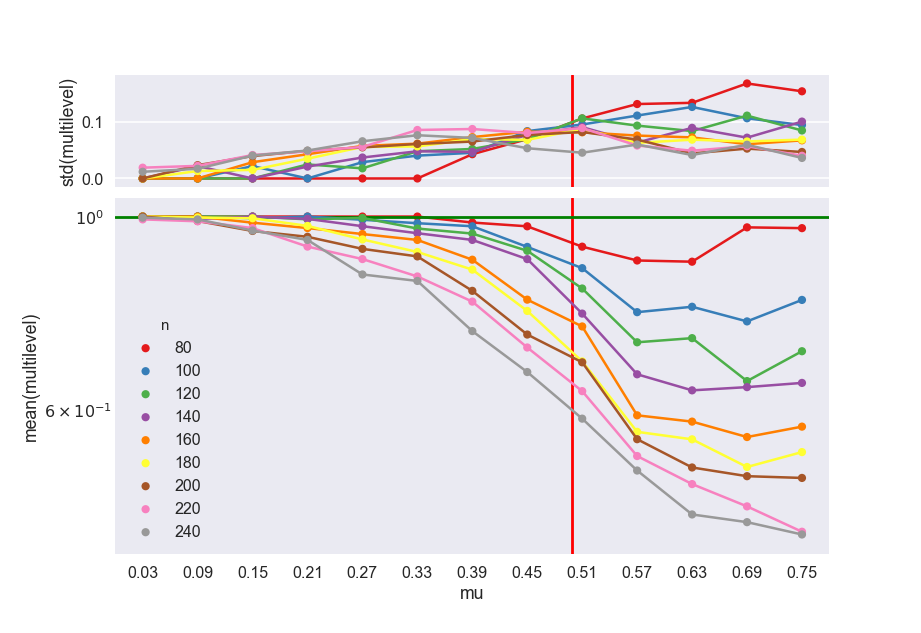
\includegraphics[width=\textwidth]{fig/ratio_vs_mu_multilevel}
        \caption{Multilevel}
        \label{fig:mouse}
    \end{subfigure}

    \begin{subfigure}[b]{0.32\textwidth}
        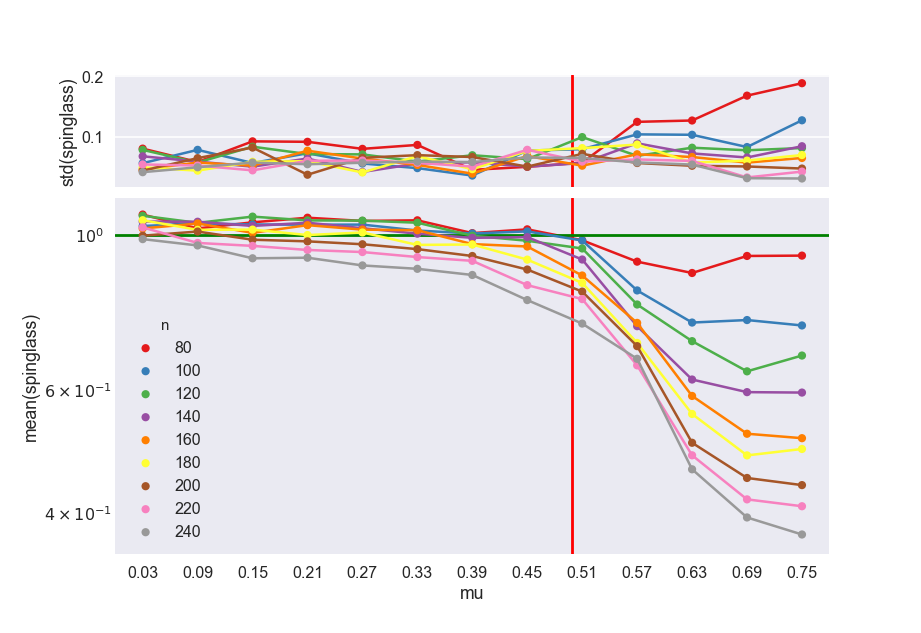
\includegraphics[width=\textwidth]{fig/ratio_vs_mu_spinglass}
        \caption{Spinglass}
        \label{fig:gull}
    \end{subfigure}
    \qquad
    %add desired spacing between images, e. g. ~, \quad, \qquad, \hfill etc. 
      %(or a blank line to force the subfigure onto a new line)
    \begin{subfigure}[b]{0.32\textwidth}
        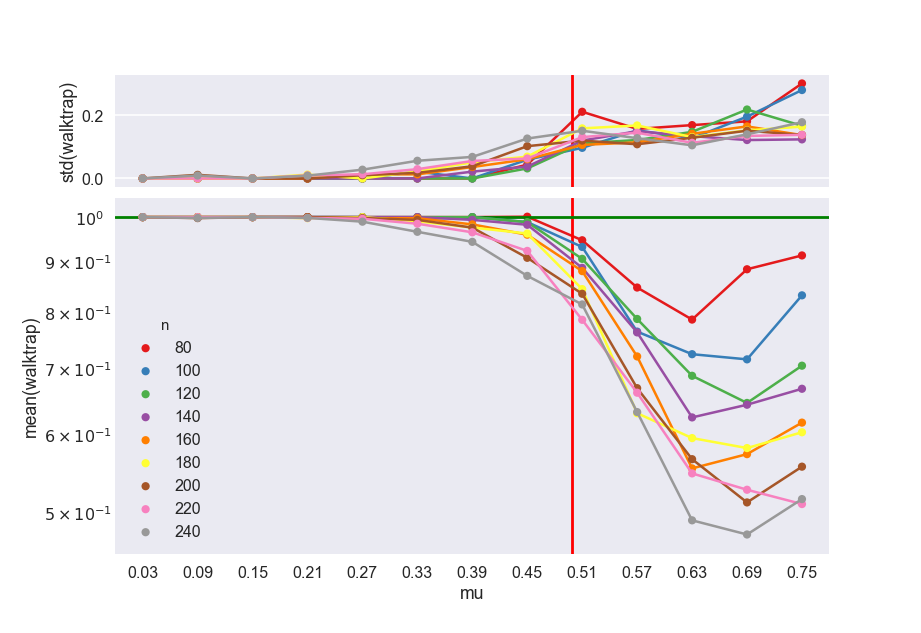
\includegraphics[width=\textwidth]{fig/ratio_vs_mu_walktrap}
        \caption{Walktrap}
        \label{fig:tiger}
    \end{subfigure}
    
    %add desired spacing between images, e. g. ~, \quad, \qquad, \hfill etc. 
    %(or a blank line to force the subfigure onto a new line)
    \begin{subfigure}[b]{0.32\textwidth}
        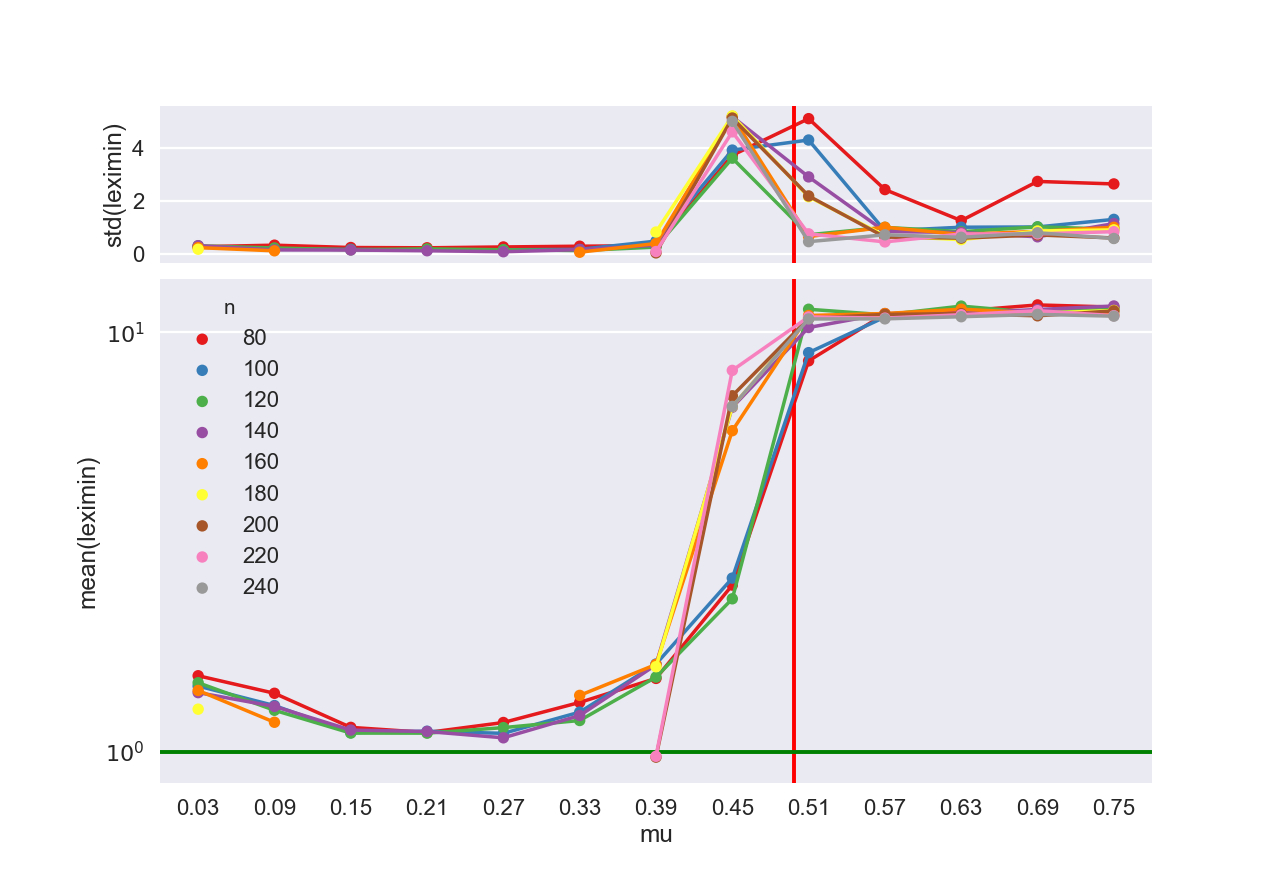
\includegraphics[width=\textwidth]{fig/ratio_vs_mu_leximin}
        \caption{Leximin}
        \label{fig:mouse}
    \end{subfigure}

  \caption{The mean ratio of detected number of communities to real number of communities defined by the LFR benchmark,~$\frac{\overline{C}}{C}$, in terms of the mixing parameter~$\mu$ on a log-linear scale. Note that the vertical axis range differs across plots. The vertical line indicates the bound on strong communities, $\mu = 0.5$. The horizontal green line shows $\overline{C} = C$.}
  \label{fig:mu_c}
\end{figure}

The final comparison we show is the computed number of communities against the true number of communities, $\overline{C}/C$. Results for each of the nine methods are shown in \autoref{fig:mu_c}. Like only the edge betweenness algorithm, the leximin method generally overestimates the number of communities that are present, and this behavior worsens for larger values of the mixing parameters. In fact, for $\mu \gtrapprox 0.57$, the identified number of communities~$\overline{C}$ is almost always equal to the number of nodes~$N$. Combined with the generally random assignments in this range, this worsening suggests that these highly interlinked networks exhibit gridlock. This suggestion is confirmed in \autoref{sec:compare_gridlock}.



\subsection{The Observed Mixing Parameter}
%
%\begin{figure}
%  \caption{The mean mixing parameter estimated by the community detection algorithm,~$\overline{\mu}$, as a function of the true mixing parameter,~$\mu$}
%  \label{fig:mu mubar}
%\end{figure}

Yang et al.\ also characterize a network in terms of the \emph{observed} mixing parameter. Because the true mixing parameter~$\mu$ can only be computed from the ground truth clustering, it is often unknown in real-world applications. An observed mixing parameter can be computed from the assigned clustering to assess the strength of computed communities. Yang et al.\ observed a general agreement between true and computed mixing parameter for all methods, until near or at the $\mu = 0.5$ threshold. The Infomap and Label propagation methods \say{fail completely} to estimate $\mu$ for larger values of $\mu$.

The leximin method breaks down, too. Gridlock occurs consistently for networks with large mixing parameters. The graph transitions from the entire graph being the community to every cluster as a singleton, where no edges are within communities. This means that $\deg^{inter}(v) =  \deg(v)$, so the observed mixing parameter for $\mu > 0.5$ is $1$.



\subsection{The Role of Network Size}

The size of the network is important, too, to the performance of a community detection algorithm. In \autoref{fig:n_nmi}, we show the NMI as a function of the network size.

\begin{figure}
\centering
    \begin{subfigure}[b]{0.32\textwidth}
        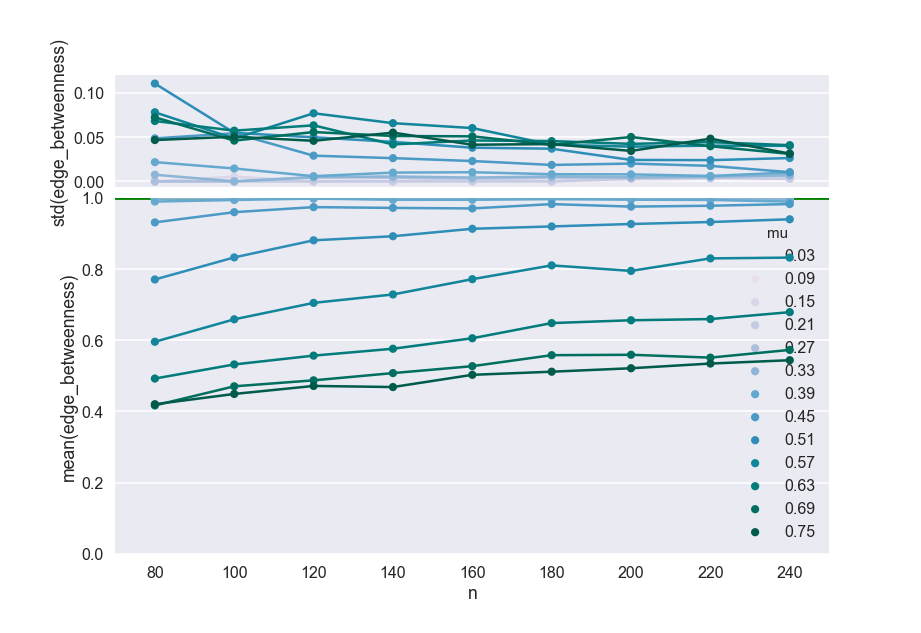
\includegraphics[width=\textwidth]{fig/nmi_vs_n_edge_betweenness}
        \caption{Edge betweenness (GN)}
        \label{fig:gull}
    \end{subfigure}
    \qquad
    %add desired spacing between images, e. g. ~, \quad, \qquad, \hfill etc. 
      %(or a blank line to force the subfigure onto a new line)
    \begin{subfigure}[b]{0.32\textwidth}
        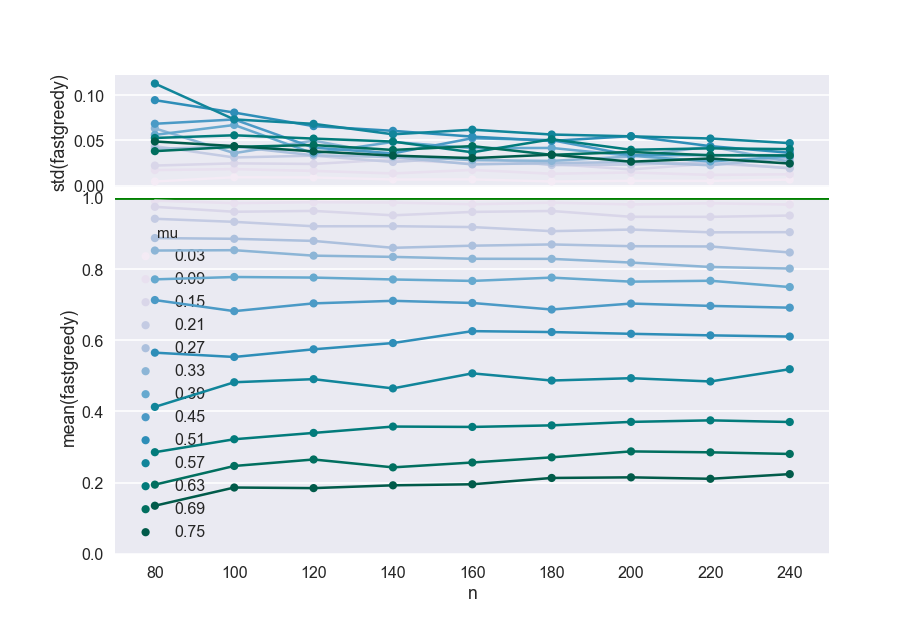
\includegraphics[width=\textwidth]{fig/nmi_vs_n_fastgreedy}
        \caption{Fastgreedy}
        \label{fig:tiger}
    \end{subfigure}
    
    %add desired spacing between images, e. g. ~, \quad, \qquad, \hfill etc. 
    %(or a blank line to force the subfigure onto a new line)
    \begin{subfigure}[b]{0.32\textwidth}
        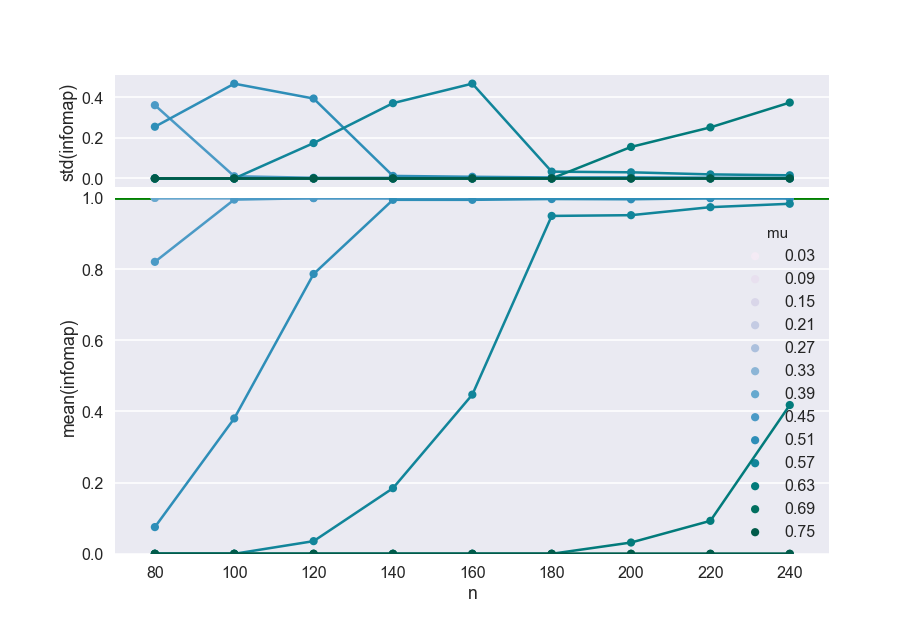
\includegraphics[width=\textwidth]{fig/nmi_vs_n_infomap}
        \caption{Infomap}
        \label{fig:mouse}
    \end{subfigure}
    \qquad
    \begin{subfigure}[b]{0.32\textwidth}
        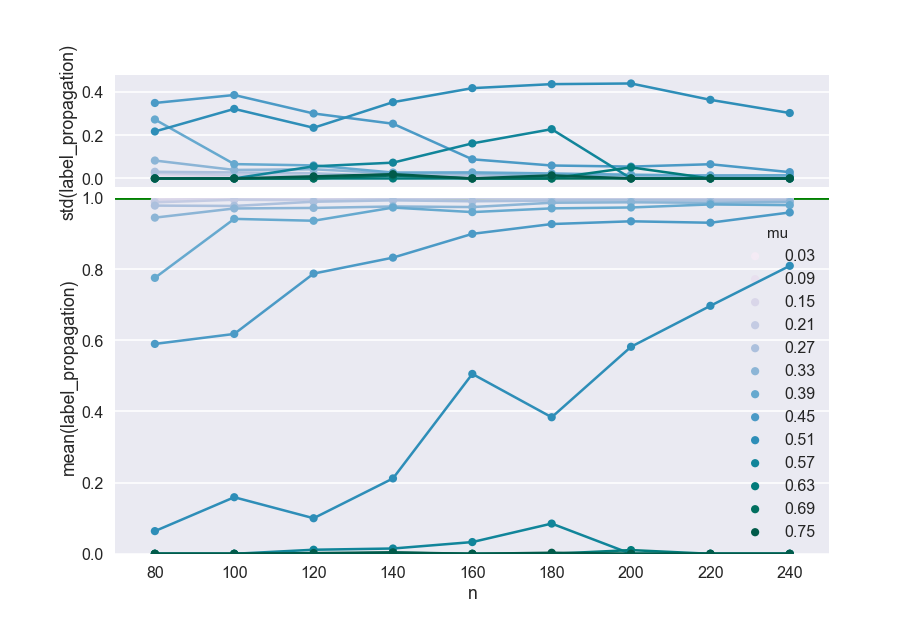
\includegraphics[width=\textwidth]{fig/nmi_vs_n_label_propagation}
        \caption{Label propagation (LPA)}
        \label{fig:gull}
    \end{subfigure}
    
    %add desired spacing between images, e. g. ~, \quad, \qquad, \hfill etc. 
      %(or a blank line to force the subfigure onto a new line)
    \begin{subfigure}[b]{0.32\textwidth}
        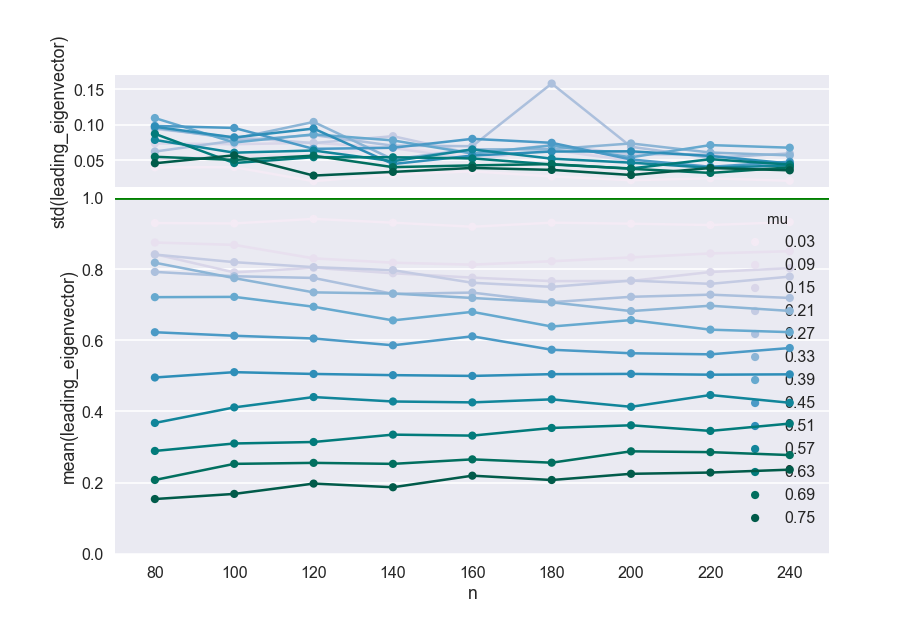
\includegraphics[width=\textwidth]{fig/nmi_vs_n_leading_eigenvector}
        \caption{Leading eigenvector}
        \label{fig:tiger}
    \end{subfigure}
    \qquad
    %add desired spacing between images, e. g. ~, \quad, \qquad, \hfill etc. 
    %(or a blank line to force the subfigure onto a new line)
    \begin{subfigure}[b]{0.32\textwidth}
        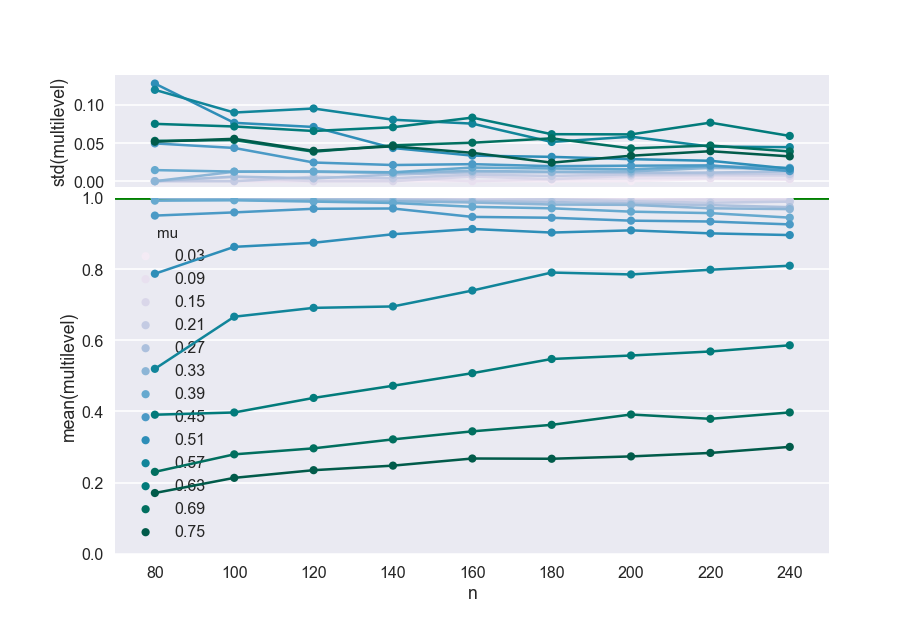
\includegraphics[width=\textwidth]{fig/nmi_vs_n_multilevel}
        \caption{Multilevel}
        \label{fig:mouse}
    \end{subfigure}

    \begin{subfigure}[b]{0.32\textwidth}
        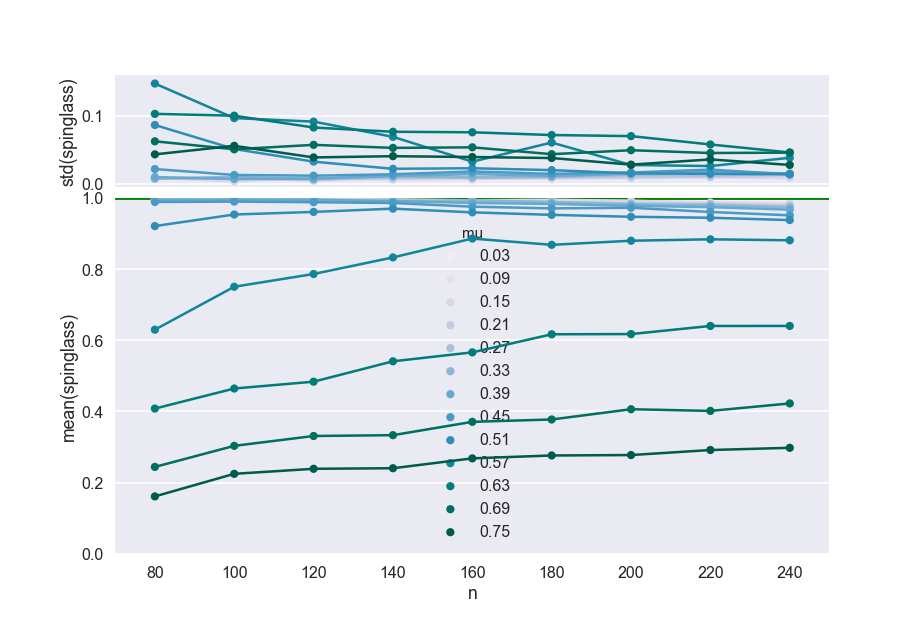
\includegraphics[width=\textwidth]{fig/nmi_vs_n_spinglass}
        \caption{Spinglass}
        \label{fig:gull}
    \end{subfigure}
    \qquad
    %add desired spacing between images, e. g. ~, \quad, \qquad, \hfill etc. 
      %(or a blank line to force the subfigure onto a new line)
    \begin{subfigure}[b]{0.32\textwidth}
        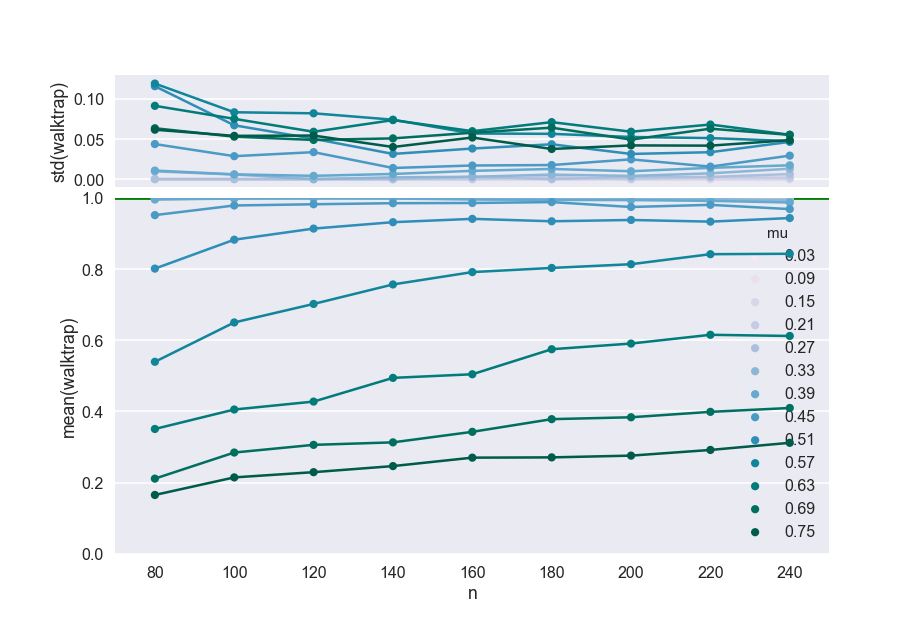
\includegraphics[width=\textwidth]{fig/nmi_vs_n_walktrap}
        \caption{Walktrap}
        \label{fig:tiger}
    \end{subfigure}

    %add desired spacing between images, e. g. ~, \quad, \qquad, \hfill etc. 
    %(or a blank line to force the subfigure onto a new line)
    \begin{subfigure}[b]{0.32\textwidth}
        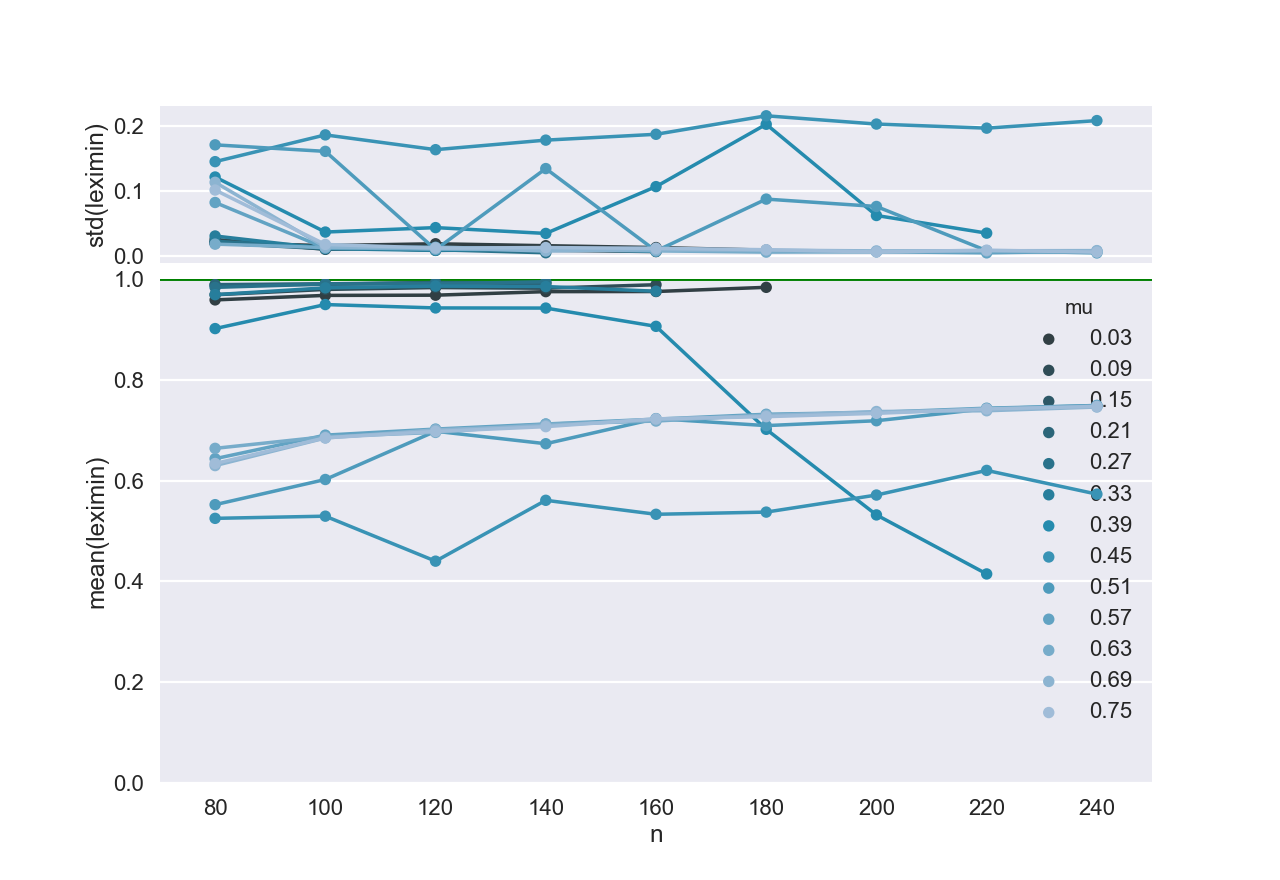
\includegraphics[width=\textwidth]{fig/nmi_vs_n_leximin}
        \caption{Leximin}
        \label{fig:mouse}
    \end{subfigure}

  \caption{The mean (top) and standard deviation (bottom) of the normalized mutual information~(NMI) as a function of the number of nodes~$N$ scale}
  \label{fig:n_nmi}
\end{figure}

The impact of network size on NMI is shown in \autoref{fig:n_nmi}. We see that in general, the size of the network does not affect the quality of the clustering when average degree and $\mu$ are fixed. The behavior of $\mu = 0.39$ is discussed later. Otherwise, whether $\mu$ is high or low, altering $N$ does not significantly affect the NMI.

\begin{figure}
	\centering
    \begin{subfigure}[b]{0.32\textwidth}
        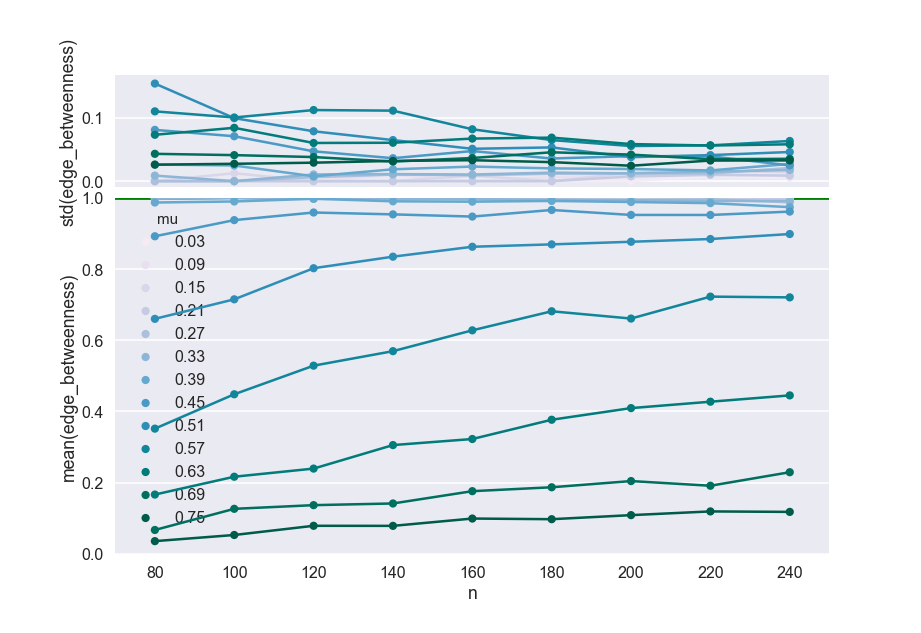
\includegraphics[width=\textwidth]{fig/ami_vs_n_edge_betweenness}
        \caption{Edge betweenness (GN)}
        \label{fig:gull}
    \end{subfigure}
    \qquad
    %add desired spacing between images, e. g. ~, \quad, \qquad, \hfill etc. 
      %(or a blank line to force the subfigure onto a new line)
    \begin{subfigure}[b]{0.32\textwidth}
        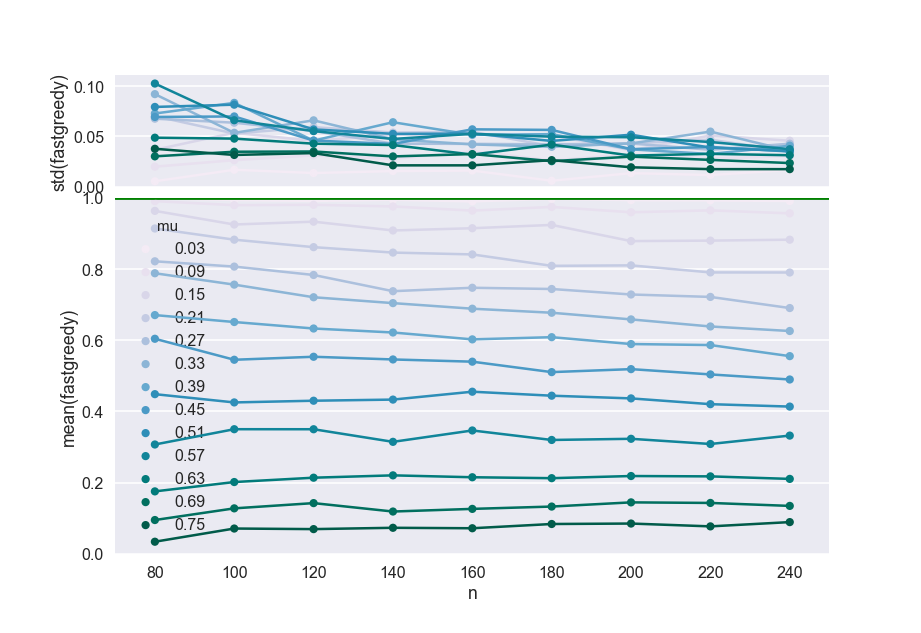
\includegraphics[width=\textwidth]{fig/ami_vs_n_fastgreedy}
        \caption{Fastgreedy}
        \label{fig:tiger}
    \end{subfigure}
    
    %add desired spacing between images, e. g. ~, \quad, \qquad, \hfill etc. 
    %(or a blank line to force the subfigure onto a new line)
    \begin{subfigure}[b]{0.32\textwidth}
        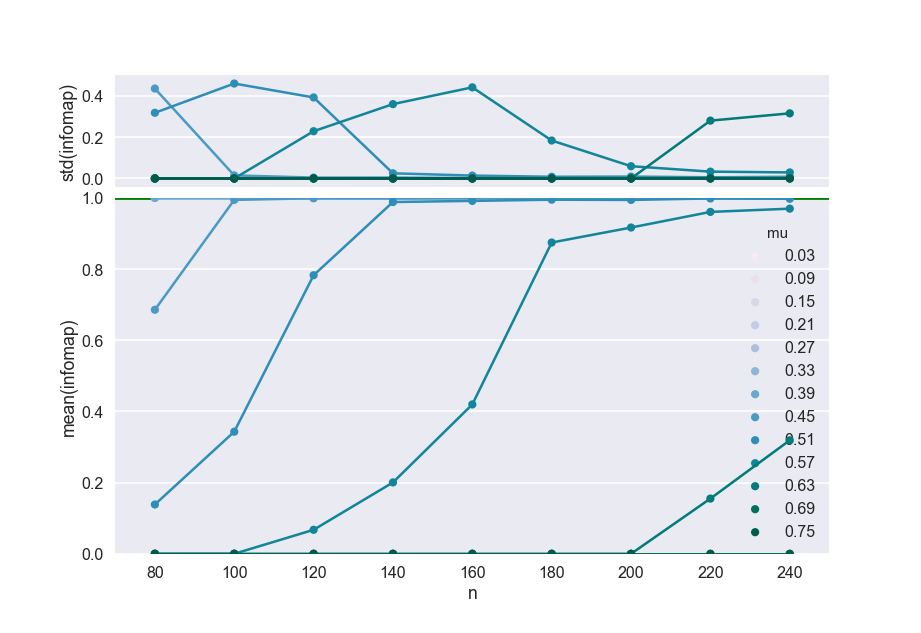
\includegraphics[width=\textwidth]{fig/ami_vs_n_infomap}
        \caption{Infomap}
        \label{fig:mouse}
    \end{subfigure}
	\qquad
    \begin{subfigure}[b]{0.32\textwidth}
        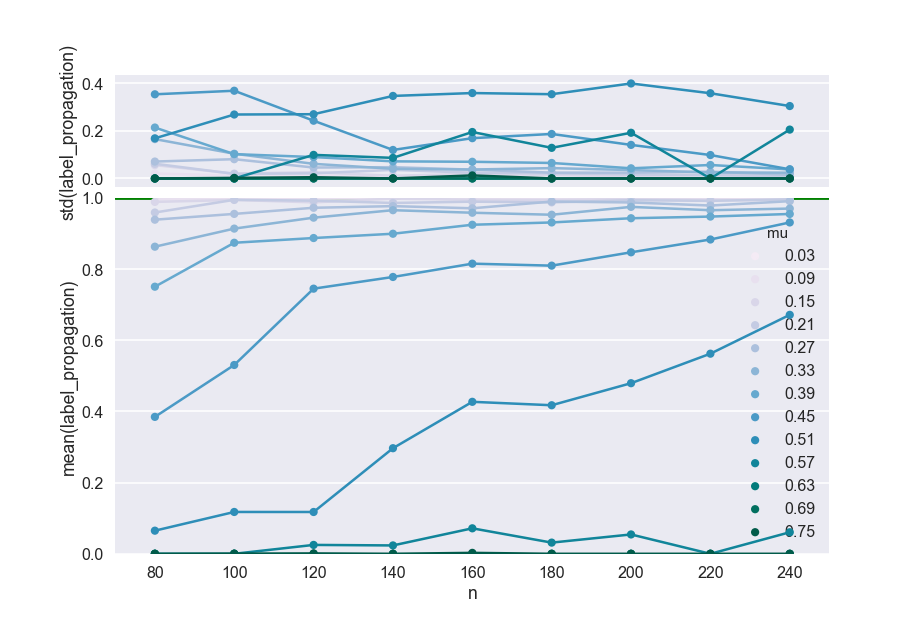
\includegraphics[width=\textwidth]{fig/ami_vs_n_label_propagation}
        \caption{Label propagation (LPA)}
        \label{fig:gull}
    \end{subfigure}
    
    %add desired spacing between images, e. g. ~, \quad, \qquad, \hfill etc. 
      %(or a blank line to force the subfigure onto a new line)
    \begin{subfigure}[b]{0.32\textwidth}
        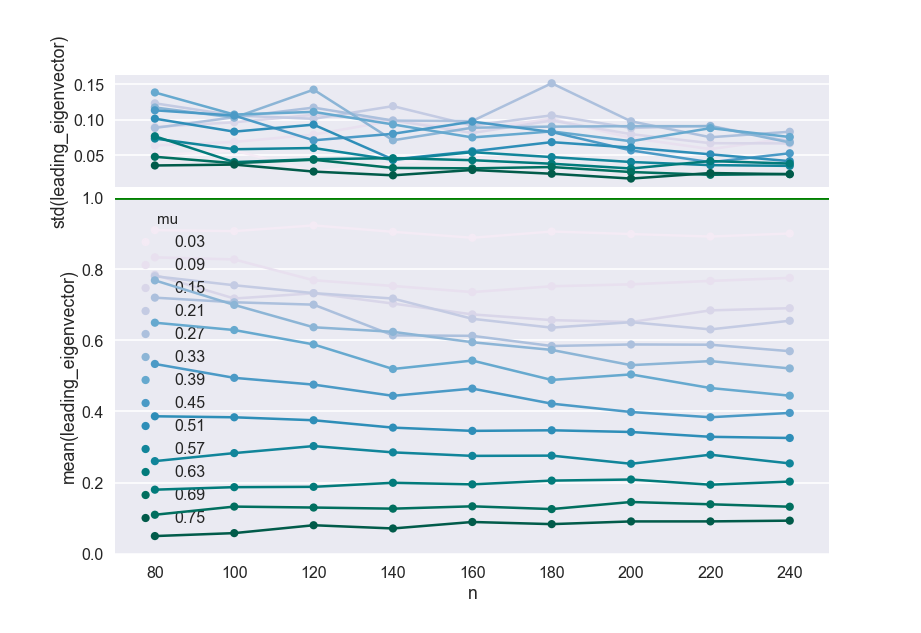
\includegraphics[width=\textwidth]{fig/ami_vs_n_leading_eigenvector}
        \caption{Leading eigenvector}
        \label{fig:tiger}
    \end{subfigure}
    \qquad
    %add desired spacing between images, e. g. ~, \quad, \qquad, \hfill etc. 
    %(or a blank line to force the subfigure onto a new line)
    \begin{subfigure}[b]{0.32\textwidth}
        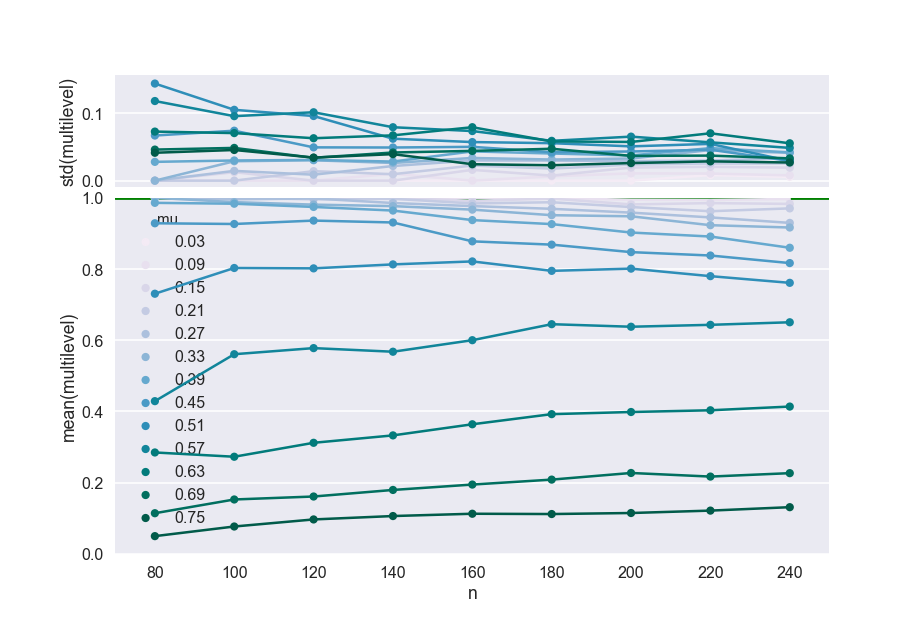
\includegraphics[width=\textwidth]{fig/ami_vs_n_multilevel}
        \caption{Multilevel}
        \label{fig:mouse}
    \end{subfigure}

    \begin{subfigure}[b]{0.32\textwidth}
        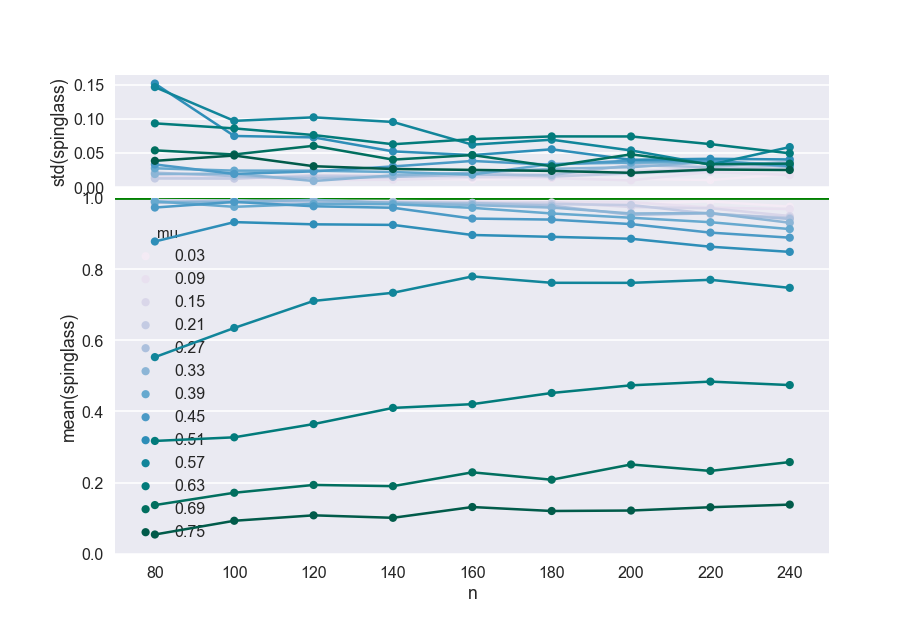
\includegraphics[width=\textwidth]{fig/ami_vs_n_spinglass}
        \caption{Spinglass}
        \label{fig:gull}
    \end{subfigure}
    \qquad
    %add desired spacing between images, e. g. ~, \quad, \qquad, \hfill etc. 
      %(or a blank line to force the subfigure onto a new line)
    \begin{subfigure}[b]{0.32\textwidth}
        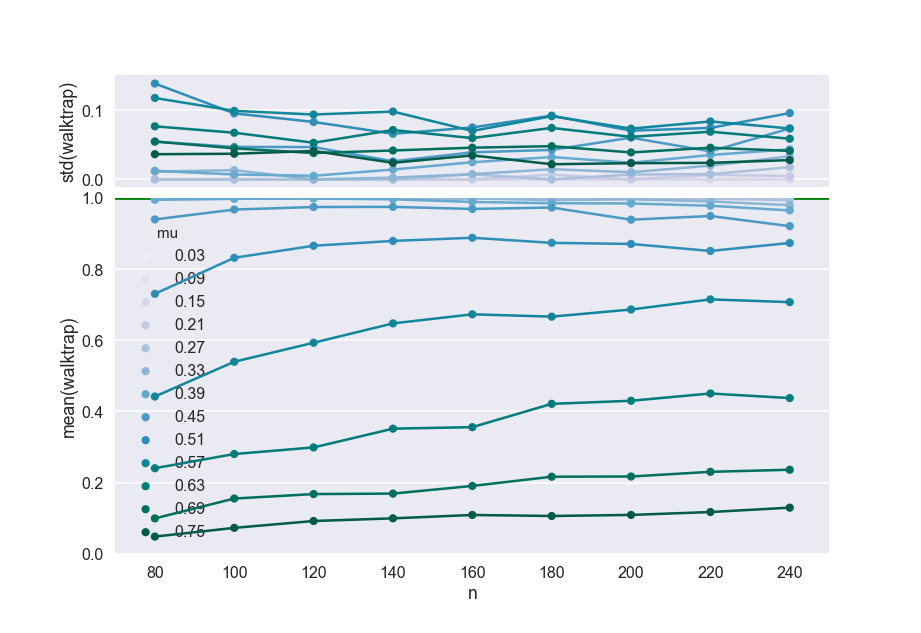
\includegraphics[width=\textwidth]{fig/ami_vs_n_walktrap}
        \caption{Walktrap}
        \label{fig:tiger}
    \end{subfigure}
    
    %add desired spacing between images, e. g. ~, \quad, \qquad, \hfill etc. 
    %(or a blank line to force the subfigure onto a new line)
    \begin{subfigure}[b]{0.32\textwidth}
        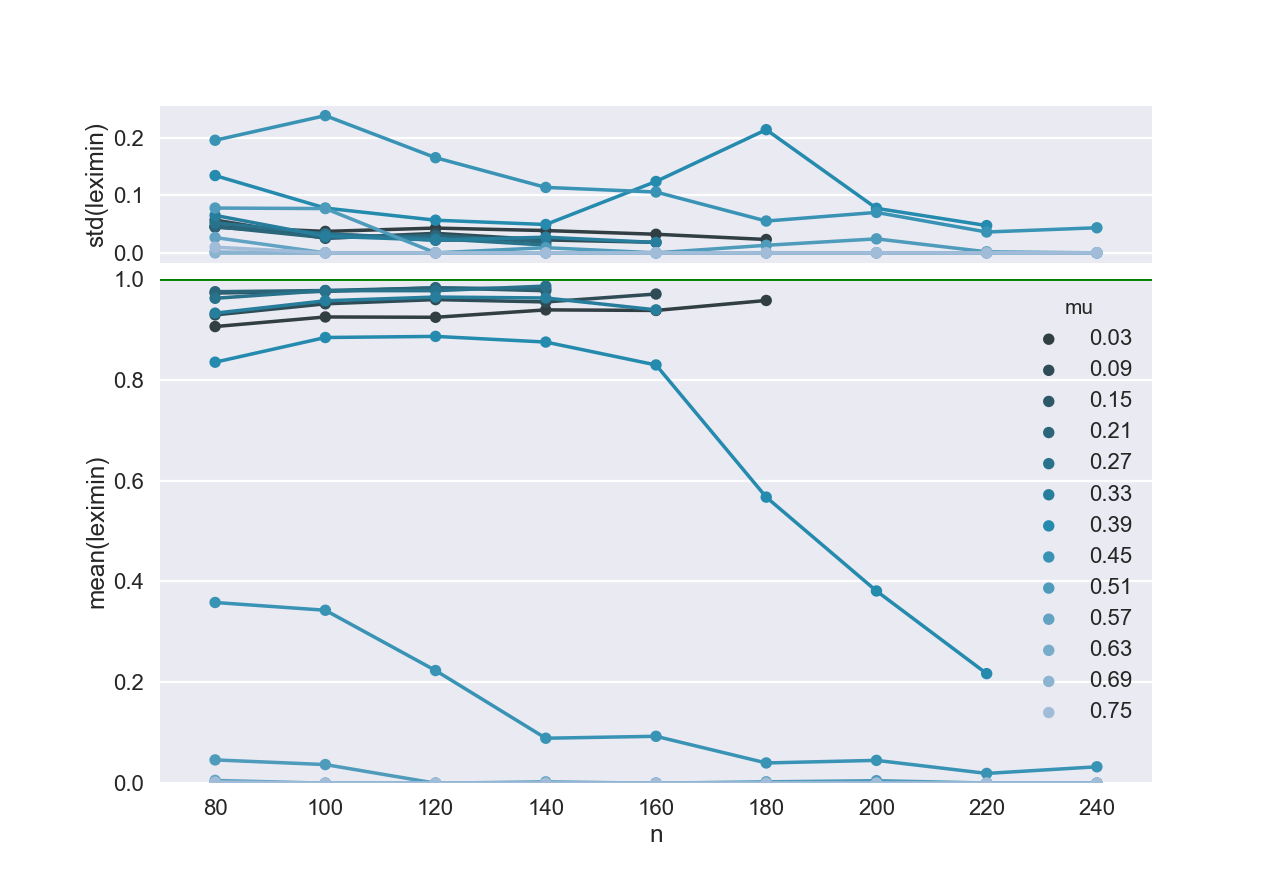
\includegraphics[width=\textwidth]{fig/ami_vs_n_leximin}
        \caption{Leximin}
        \label{fig:mouse}
    \end{subfigure}

  \caption{The mean (top) and standard deviation (bottom) of the adjusted mutual information~(AMI) as a function of the number of nodes~$N$ scale}
  \label{fig:n_ami}
\end{figure}

The AMI shows similar patterns for varying $N$. \autoref{fig:n_ami} shows that for a fixed mixing parameter~$\mu$, network size tends not to change the AMI. Of course, for high $\mu$, the AMI is dramatically lower, tending to be near 0. This is again because NMI does not adjust for good fortune in cluster assignments due to chance. The drop in performance of $\mu=0.39$ is even more pronounced. 

\begin{figure}
	\centering

    \begin{subfigure}[b]{0.32\textwidth}
        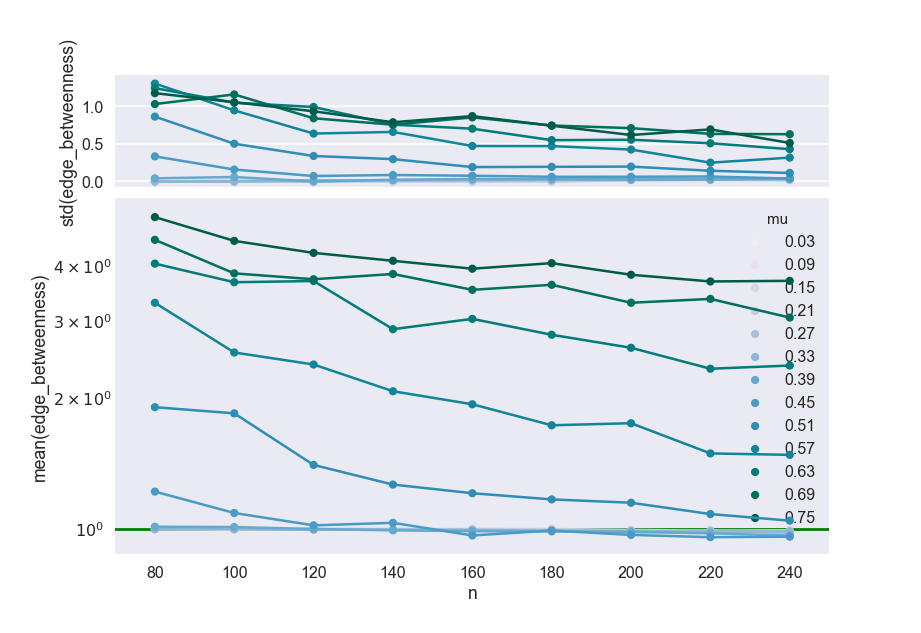
\includegraphics[width=\textwidth]{fig/ratio_vs_n_edge_betweenness}
        \caption{Edge betweenness (GN)}
        \label{fig:gull}
    \end{subfigure}
    \qquad
    %add desired spacing between images, e. g. ~, \quad, \qquad, \hfill etc. 
      %(or a blank line to force the subfigure onto a new line)
    \begin{subfigure}[b]{0.32\textwidth}
        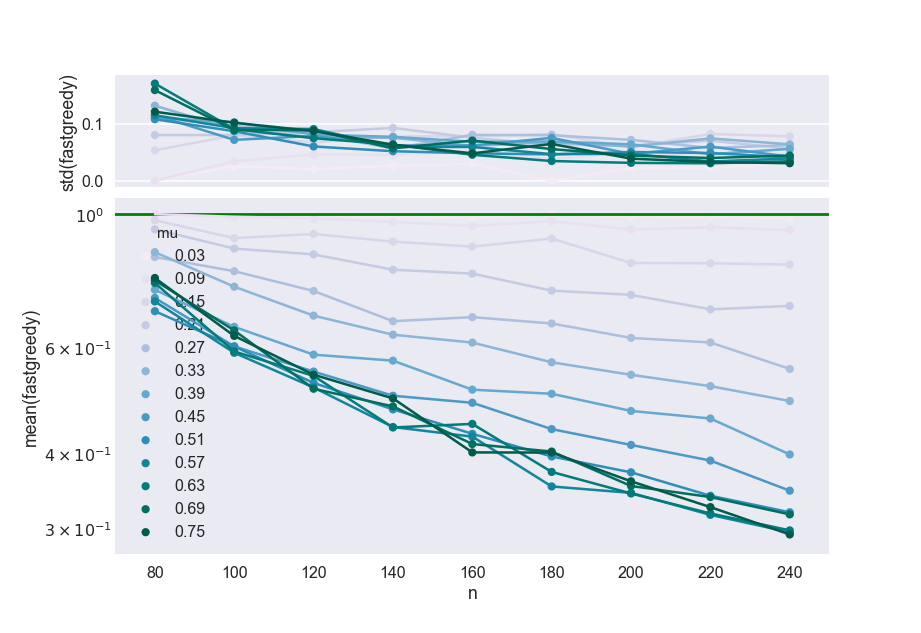
\includegraphics[width=\textwidth]{fig/ratio_vs_n_fastgreedy}
        \caption{Fastgreedy}
        \label{fig:tiger}
    \end{subfigure}
    
    %add desired spacing between images, e. g. ~, \quad, \qquad, \hfill etc. 
    %(or a blank line to force the subfigure onto a new line)
    \begin{subfigure}[b]{0.32\textwidth}
        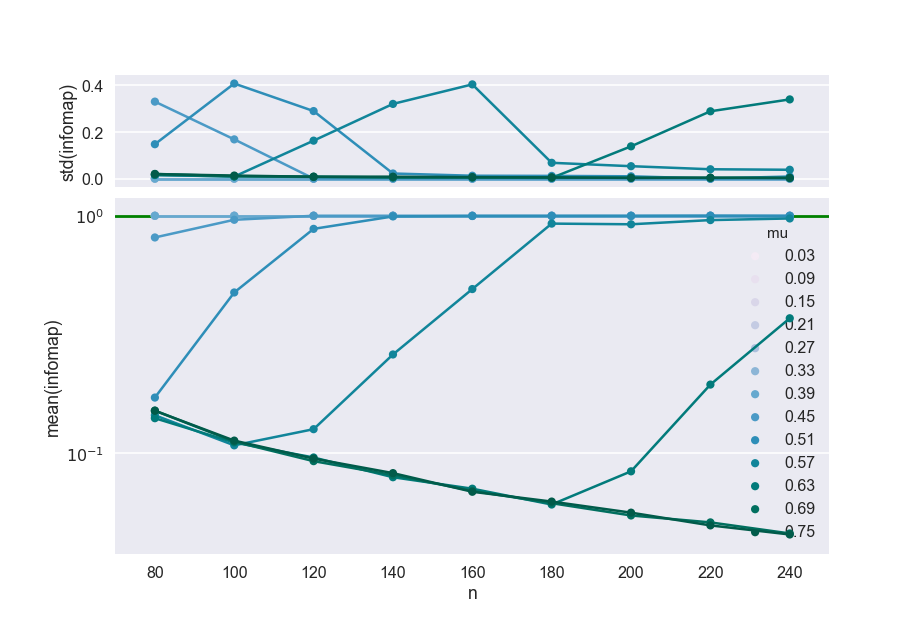
\includegraphics[width=\textwidth]{fig/ratio_vs_n_infomap}
        \caption{Infomap}
        \label{fig:mouse}
    \end{subfigure}
    \qquad
    \begin{subfigure}[b]{0.32\textwidth}
        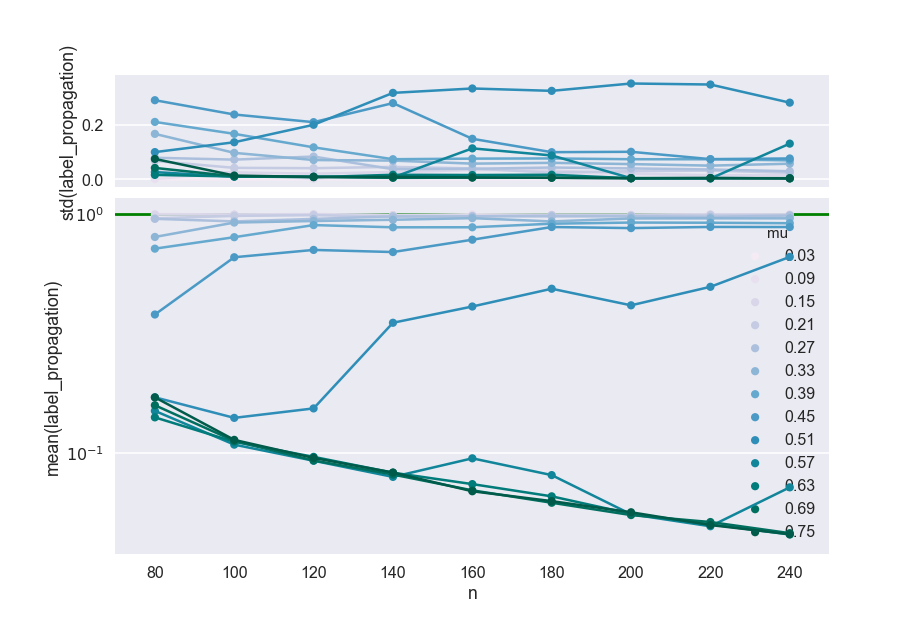
\includegraphics[width=\textwidth]{fig/ratio_vs_n_label_propagation}
        \caption{Label propagation (LPA)}
        \label{fig:gull}
    \end{subfigure}
    
    %add desired spacing between images, e. g. ~, \quad, \qquad, \hfill etc. 
      %(or a blank line to force the subfigure onto a new line)
    \begin{subfigure}[b]{0.32\textwidth}
        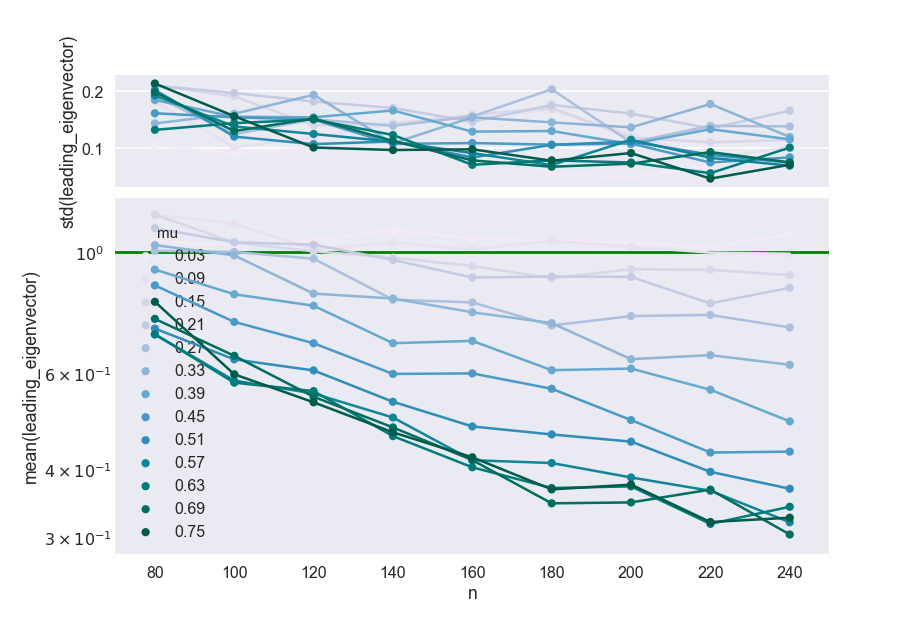
\includegraphics[width=\textwidth]{fig/ratio_vs_n_leading_eigenvector}
        \caption{Leading eigenvector}
        \label{fig:tiger}
    \end{subfigure}
    %add desired spacing between images, e. g. ~, \quad, \qquad, \hfill etc. 
    %(or a blank line to force the subfigure onto a new line)
    \qquad
    \begin{subfigure}[b]{0.32\textwidth}
        \includegraphics[width=\textwidth]{fig/ratio_vs_n_multilevel}
        \caption{Multilevel}
        \label{fig:mouse}
    \end{subfigure}

    \begin{subfigure}[b]{0.32\textwidth}
        \includegraphics[width=\textwidth]{fig/ratio_vs_n_spinglass}
        \caption{Spinglass}
        \label{fig:gull}
    \end{subfigure}
    \qquad
    %add desired spacing between images, e. g. ~, \quad, \qquad, \hfill etc. 
      %(or a blank line to force the subfigure onto a new line)
    \begin{subfigure}[b]{0.32\textwidth}
        \includegraphics[width=\textwidth]{fig/ratio_vs_n_walktrap}
        \caption{Walktrap}
        \label{fig:tiger}
    \end{subfigure}
    
    %add desired spacing between images, e. g. ~, \quad, \qquad, \hfill etc. 
    %(or a blank line to force the subfigure onto a new line)
    \begin{subfigure}[b]{0.32\textwidth}
        \includegraphics[width=\textwidth]{fig/ratio_vs_n_leximin}
        \caption{Leximin}
        \label{fig:mouse}
    \end{subfigure}

  \caption{The mean of the detected number of communities over the real number of communities defined by the LFR benchmark,~$\frac{\overline{C}}{C}$, in terms of the network size~$N$ on a log-linear scale. Note that the vertical axis range differs across plots. The horizontal green line shows $\overline{C} = C$.}
  \label{fig:n_c}
\end{figure}

Finally, we reconsider the ratio of computed communities to true communities, this time from the frame of network size. The accuracy of the nine methods is shown in \autoref{fig:n_c}. For low values of the mixing parameter, the method slightly overestimates the number of clusters. For higher values, the mean ratio is equal to the cap on the number of communities defined by the LFR parameterization---we're producing singleton clusterings. We can see the transition between behaviors at $\mu \approx 0.4$. By contrast to the leximin method, other methods' performance seems to falter as networks grow larger. Edge betweenness and leximin are the only two that show no reliable accuracy gap as a result of network size.


\subsection{Gridlock} \label{sec:compare_gridlock}

\begin{figure}
	\centering
    \begin{subfigure}[b]{0.30\textwidth}
        \includegraphics[width=\textwidth]{fig/count_vs_mu}
        \caption{Number of terminating benchmarks}
        \label{fig:gull}
    \end{subfigure}
    ~%add desired spacing between images, e. g. ~, \quad, \qquad, \hfill etc. 
      %(or a blank line to force the subfigure onto a new line)
    \begin{subfigure}[b]{0.30\textwidth}
        \includegraphics[width=\textwidth]{fig/gridlock_vs_mu}
        \caption{Number of benchmarks resulting in gridlock}
        \label{fig:tiger}
    \end{subfigure}
    ~%add desired spacing between images, e. g. ~, \quad, \qquad, \hfill etc. 
    %(or a blank line to force the subfigure onto a new line)
    \begin{subfigure}[b]{0.30\textwidth}
        \includegraphics[width=\textwidth]{fig/rate_vs_mu}
        \caption{Proportion of benchmarks with gridlock}
        \label{fig:mouse}
    \end{subfigure}

  \caption{Gridlock, in terms of the mixing parameter~$\mu$. The vertical red line indicates the boundary between strong and weak communities, $\mu = 0.5$. The green horizontal line always represents the 100\% mark.}
  \label{fig:mu_gridlock}
\end{figure}

\begin{figure}
	\centering
    \begin{subfigure}[b]{0.30\textwidth}
        \includegraphics[width=\textwidth]{fig/count_vs_n}
        \caption{Number of terminating benchmarks}
        \label{fig:gull}
    \end{subfigure}
    ~%add desired spacing between images, e. g. ~, \quad, \qquad, \hfill etc. 
      %(or a blank line to force the subfigure onto a new line)
    \begin{subfigure}[b]{0.30\textwidth}
        \includegraphics[width=\textwidth]{fig/gridlock_vs_n}
        \caption{Number of benchmarks resulting in gridlock}
        \label{fig:tiger}
    \end{subfigure}
    ~%add desired spacing between images, e. g. ~, \quad, \qquad, \hfill etc. 
    %(or a blank line to force the subfigure onto a new line)
    \begin{subfigure}[b]{0.30\textwidth}
        \includegraphics[width=\textwidth]{fig/rate_vs_n}
        \caption{Proportion of benchmarks with gridlock}
        \label{fig:mouse}
    \end{subfigure}

  \caption{Gridlock, in terms of the network size~$N$. The green horizontal line always represents the 100\% mark.}
  \label{fig:n_gridlock}
\end{figure}

Gridlock in the leximin method means that we have one flat clustering that fragments into individual node communities where all edges are at capacity in the sense of flow on the paths identified by a particular solution. It represents a failure of the leximin method to identify any mesoscopic, community structure. The work in \autoref{ch:random} shows that this is a reasonable conclusion. Gridlock is recognized in the first subproblem, allowing the method to \say{fail fast} when it does not detect a community structure.

This \say{failing fast} introduces a non-response bias in our results~\cite{armstrong1977estimating}. Networks that gridlock only need to compute one iteration of the hierarchical MCFP. In general, the number of iterations can be as high as $N-1$, so networks without gridlock will take longer to execute than those with gridlock. These networks are filtered out by the upper bound on computing time for a single job. 

Networks without gridlock have an identified community structure, so this non-response bias inflates the mean ratio of computed communities to true communities, while depressing the average AMI.

In \autoref{fig:mu_gridlock}, we see that for every large network, gridlock occurs. Further, there's a tendency for networks with low $\mu$ to fail to complete, taking more than the allowed time to identify structure. Interestingly, for $N \in \{160, 180\}$, the execution nearly always completes for small $\mu$. A mixing parameter of $\mu \approx0.25$ produces networks with deeper structure, then. This warrants future investigation. 

Gridlock is consistently absent from networks with very strong communities, and it becomes more prevalent as ties between communities grow. \autoref{fig:n_gridlock} shows that there is little dependence on network size, so this seems to be a general property of networks. This has implications for traffic theory: by increasing the number of routes between communities, bottlenecks are reduced until the entire network becomes one giant community. This suggests the ability to reduce the frequency of bottlenecks by reducing community structure, introducing not only large capacity between communities but multiple points of contact between each community.

\section{Running Time}

Three practical implementation factors prevent us from adequately comparing the runtime of the leximin method to the other clustering techniques. Most importantly, the implementation of the leximin algorithm does not perform a \say{warm start}: at each level, rather than restarting at the previous solution, it starts at the base initialization again. This inflates the actual runtime relative to an ideal implementation. Second, the algorithms are implemented in different languages. The \say{igraph} package is implemented in C with interfaces to Python and R, whereas the leximin method is written in AMPL. Finally, with a fixed amount of computation time on the compute cluster for a single job, only the large networks that exhibit gridlock (suggesting no strong community structure) could finish executing.

That being said, it is clear that the leximin method is much slower than the other methods. As discussed in \autoref{sec:complexity and size}, the method runs in a high-order polynomial time, unlike the popular methods which run in $O(N^5)$ at worst for dense graphs. For a single medium-sized network, the implementation may not finish in the span of 3 hours.  By contrast, all eight other methods combined can be run \emph{in serial} on the entire battery of benchmark graphs used in this thesis in about 3 hours. They have been tested on networks with up to millions of nodes~\cite{hric2014community}, while the leximin method is restricted to those with a few hundred.

\section{Discussion}

\begin{figure}
\centering
\includegraphics[height=0.4\textheight]{fig/krebs}
\caption{Krebs's 9/11 hijacker network. One actor, Imad Eddin Barakat Yarkas, is indicated with a blue line. He has two connections to each of two communities, so as the leximin method proceeds, he becomes isolated by a pair of sparsest cuts, separated from any communities.}
\label{fig:krebs}
\end{figure}

For high values of the mixing parameter, the NMI of the leximin method outperforms all other methods. This does not mean that the leximin method is superior in this case. Rather, the leximin allocation of flow produces gridlock, especially at larger network sizes. The singleton clustering of gridlock does not capture the intended structure of the LFR benchmark graphs, yet the leximin method scores highly. AMI ameliorates this discrepancy, and it is a reasonable measurement for the community to use moving forward. 

Even when it is not gridlocking, the leximin method consistently achieves a slightly lower AMI than, say, the Walktrap method. Further, it overestimates the number of clusters in nearly every case. This is attributable to a tendency to splinter off small subgraphs (e.g.\ singletons) which lack strong connections to their assigned community---rather than assigning to incorrect clusters. The contingency table in \autoref{tab:crosstab} supports this idea, and Lemma~\label{lemma:modularity} explains why this behavior impedes maximization of modularity.

A real-world example also supports the idea that the leximin method splinters off small groups, and it suggests that this occurs when nodes are well-connected to multiple communities. In Krebs's 9/11 hijacker network (shown in \autoref{fig:krebs})~\cite{krebs2002uncloaking}, Imad Eddin Barakat Yarkas has four connections: two each to two dense regions. In one iteration of the leximin algorithm, he is separated from one of these communities, and he is separated from the other in the immediately succeeding iteration. This suggests that he has a role as a hub or middleman between the groups. Similar structures in LFR graphs will also produce singleton clusters, separating hubs from firm communities. The leximin algorithm is penalized for its ability to identify these members of overlapping flat communities, because the LFR benchmark does not specify overlapping communities. 

Two of the LFR benchmark's three creators have proposed an extension to networks with overlapping communities~\cite{lancichinetti2009benchmarks}. Future work can explore the accuracy of the leximin method on this benchmark, compared to other algorithms that identify overlapping communities.

%\section{Introduction}
%
%There is no consensus on the definition of a \say{community}~\cite{hu2008comparative}, which may contribute to the multitude of extant methods: Each may be best-suited for its own notion of a community. Radicchi et al. provide a pair of definitions~\cite{radicchi2004defining}: a \emph{strong} community, in which \emph{each} node has more intra-community than inter-community connections, and a \emph{weak} community, where the \emph{average} intra-community degree exceeds the \emph{average} inter-community degree. This motivates the \emph{mixing parameter}, $\mu$~\cite{orman2009comparison}. 
%
%The mixing parameter, computed as
%\begin{equation}  \label{eq:mixing parameter}
%%
%\mu = \frac{\sum_{v \in V}\deg^{inter}(v)}{\sum_{v \in V}\deg(v)}
%%
%\end{equation}
%relates the inter-community degree~$\deg^{inter}(v)$ to the node's total degree~$\deg(v)$. When $\mu > \frac{1}{2}$, strong communities cannot exist~\cite{yang2016comparative}\todo{In the LFR benchmark. This is because it assumes a uniform $\mu$ for all nodes.}.
%
%\subsection{The MCF Cut Algorithm}
%
%Mann's algorithm works by computing $k$-partite cuts determined by the saturation of edges. When maximizing throughput between all pairs, a set of \emph{critical edges} will become fully saturated, corresponding to the idea of \emph{breakdown} in traffic theory: \say{the onset of congested traffic in an initial free traffic flow}~\cite{kerner2009traffic}. Matula showed that these critical, saturated edges partition the graph into 2 or more subgraphs. Mann does this hierarchically, using the flow of the solution as the starting point and maximizing throughput until the next set of edges is saturated. This is shown in \autoref{alg:hmcfp}.
%%%
%\subsection{Evaluation of Clustering Against Ground Truth}
%
%Mann proposed a metric~$M$ for scoring the partition of a network into communities against a ground truth. Objecting to the use of vertex set membership metrics, he proposed to use the accuracy score of a binary classification of edges as inter- or intra-community edges. He used this evaluation to show the superiority of the maximin algorithm over the edge betweenness algorithm of Girvan and Newman, which repeatedly removes the most \say{between} edge, potentially removing edges within an identified cluster. As the maximin algorithm cannot remove an edge within a community\todo{Do I need to prove this?}, the GN algorithm can receive a lower score while identifying the same communities. Further, the $M$~score's \say{sensitivity} to edges is irrelevant in other techniques which do not rely on edge removal. The metric seems specifically tailored to penalize the GN algorithm.
%